%        File: arfc-beamer.tex
%     Created: Sun May 5 10:00 PM 2013 C
%


%\documentclass[11pt,handout]{beamer}
\documentclass[9pt]{beamer}
\usetheme[white]{Illinois}
\title[Short Title]{Fluoride-Salt-Cooled High-Temperature Reactor Design Optimization with Evolutionary Algorithms \\ Preliminary Exam}
\author[Your Name]{Gwendolyn J.Y. Chee}
\date[09.13.2021]{September 13, 2021}
\institute{
Dept. of Nuclear, Plasma and Radiological Engineering \\ University of Illinois at Urbana-Champaign
}

%\usepackage{bbding}
\usepackage{amsfonts}
\usepackage{amsmath}
\usepackage{xspace}
\usepackage{graphicx}
\usepackage{booktabs} % nice rules for tables
\usepackage{microtype} % if using PDF
\usepackage{bigints}
\usepackage{minted}

\newcommand{\Cyclus}{\textsc{Cyclus}\xspace}%
\newcommand{\Cycamore}{\textsc{Cycamore}\xspace}%
\newcommand{\deploy}{\texttt{d3ploy}\xspace}%
\newcommand{\units}[1] {\:\text{#1}}%
\newcommand{\SN}{S$_N$}%{S$_\text{N}$}%{$S_N$}%
\DeclareMathOperator{\erf}{erf}
%I need some complimentary error funcitons... 
\DeclareMathOperator{\erfc}{erfc}
%page numbers
\setbeamertemplate{footline}[page number]
\setbeamertemplate{caption}[numbered]
%Those icons in the references are terrible looking
\setbeamertemplate{bibliography item}[text]

\usepackage{tkz-euclide}
\usepackage{tikz}
\usetikzlibrary{positioning, arrows, decorations, shapes}

\usetikzlibrary{shapes.geometric,arrows}
\tikzstyle{process} = [rectangle, rounded corners, minimum width=3cm, minimum height=1cm,text centered, draw=black, fill=blue!30]
\tikzstyle{object} = [ellipse, rounded corners, minimum width=3cm, minimum height=1cm,text centered, draw=black, fill=green!30]
\tikzstyle{arrow} = [thick,->,>=stealth]

\definecolor{illiniblue}{HTML}{B1C6E2}
\definecolor{illiniorange}{HTML}{f8c2a2}
\definecolor{illinigreen}{HTML}{a0deb1}
\definecolor{grey}{HTML}{dce3de}
\usetikzlibrary{shapes.geometric, arrows}
\tikzstyle{oblock} = [rectangle, draw, fill=illiniorange, 
text width=9em, text centered, rounded corners, minimum height=4em]
\tikzstyle{bblock} = [rectangle, draw, fill=illiniblue, 
text width=8em, text centered, rounded corners, minimum height=4em]
\tikzstyle{gblock} = [rectangle, draw, fill=illinigreen, 
text width=8em, text centered, rounded corners, minimum height=4em]
\tikzstyle{lgblock} = [rectangle, draw, fill=illinigreen, 
text width=9em, text centered, rounded corners, minimum height=4em]
\tikzstyle{noblock} = [rectangle,
text width=8em, text centered, minimum height=4em]
\tikzstyle{greyblock} = [rectangle, fill=grey, 
text width=8em, minimum height=4em, rounded corners]
\tikzstyle{lgreyblock} = [rectangle, fill=grey, 
text width=9em, minimum height=4em, rounded corners]
\tikzstyle{llgreyblock} = [rectangle, fill=grey, 
text width=20em, minimum height=4em, rounded corners]
\tikzstyle{arrow} = [thick,->,>=stealth]

\definecolor{fhrblue}{HTML}{0000ff}
\definecolor{fhrgrey}{HTML}{808080}
\definecolor{fhrred}{HTML}{f10a0a}
\definecolor{fhrgreen}{HTML}{2f6d39}
\definecolor{fhryellow}{HTML}{fdfe36}

\usepackage{tabularx}
\newcolumntype{b}{>{\hsize=1.0\hsize}X}
\newcolumntype{s}{>{\hsize=.5\hsize}X}
\newcolumntype{m}{>{\hsize=.75\hsize}X}
\newcolumntype{x}{>{\hsize=.25\hsize}X}
\newcolumntype{L}{>{\raggedright\arraybackslash}X}
\newcolumntype{R}{>{\raggedleft\arraybackslash}X}
\def\arraystretch{1}
%%%% Acronym support
\usepackage{multirow}
\usepackage{graphicx}
\usepackage{subcaption}

\usepackage[acronym,toc]{glossaries}
%\newacronym{<++>}{<++>}{<++>}
\newacronym[longplural={metric tons of heavy metal}]{MTHM}{MTHM}{metric ton of heavy metal}
\newacronym{3D CAD}{3D CAD}{three-dimensional Computer-Aided Design}
\newacronym{ABM}{ABM}{agent-based modeling}
\newacronym{ACDIS}{ACDIS}{Program in Arms Control \& Domestic and International Security}
\newacronym{AHTR}{AHTR}{Advanced High Temperature Reactor}
\newacronym{AI}{AI}{Artificial Intelligence}
\newacronym{AM}{AM}{Additive Manufacturing}
\newacronym{AMAFT}{AMAFT}{Additive Manufacturing as an Alternative Fabrication Technique}
\newacronym{ANDRA}{ANDRA}{Agence Nationale pour la gestion des D\'echets RAdioactifs, the French National Agency for Radioactive Waste Management}
\newacronym{ANL}{ANL}{Argonne National Laboratory}
\newacronym{ANS}{ANS}{American Nuclear Society}
\newacronym{API}{API}{application programming interface}
\newacronym{ARE}{ARE}{Aircraft Reactor Experiment}
\newacronym{ARFC}{ARFC}{Advanced Reactors and Fuel Cycles}
\newacronym{ARMA}{ARMA}{Autoregressive Moving Average}
\newacronym{ARCH}{ARCH}{Autoregressive Heteroskedasticity}
\newacronym{ARIMA}{ARIMA}{Auto-Regressive Integrated Moving Averages}
\newacronym{ASME}{ASME}{American Society of Mechanical Engineers}
\newacronym{ATWS}{ATWS}{Anticipated Transient Without Scram}
\newacronym{BDBE}{BDBE}{Beyond Design Basis Event}
\newacronym{BIDS}{BIDS}{Berkeley Institute for Data Science}
\newacronym{BNL}{BNL}{Brookhaven National Laboratory}
\newacronym{CAFCA}{CAFCA}{ Code for Advanced Fuel Cycles Assessment }
\newacronym{CDTN}{CDTN}{Centro de Desenvolvimento da Tecnologia Nuclear}
\newacronym{CFD}{CFD}{Computational Fluid Dynamics}
\newacronym{CEA}{CEA}{Commissariat \`a l'\'Energie Atomique et aux \'Energies Alternatives}
\newacronym{CI}{CI}{continuous integration}
\newacronym{CIEMAT}{CIEMAT}{Centro de Investigaciones Energéticas, Medioambientales y Tecnológicas}
\newacronym{CNEN}{CNEN}{Comiss\~{a}o Nacional de Energia Nuclear}
\newacronym{CNERG}{CNERG}{Computational Nuclear Engineering Research Group}
\newacronym{CNRS}{CNRS}{Le Centre National De La Recherche Scientifique}
\newacronym{COSI}{COSI}{Commelini-Sicard}
\newacronym{COTS}{COTS}{commercial, off-the-shelf}
\newacronym{CSNF}{CSNF}{commercial spent nuclear fuel}
\newacronym{CTAH}{CTAHs}{Coiled Tube Air Heaters}
\newacronym{CUBIT}{CUBIT}{CUBIT Geometry and Mesh Generation Toolkit}
\newacronym{CURIE}{CURIE}{Centralized Used Fuel Resource for Information Exchange}
\newacronym{DAG}{DAG}{directed acyclic graph}
\newacronym{DANESS}{DANESS}{Dynamic Analysis of Nuclear Energy System Strategies}
\newacronym{DBE}{DBE}{Design Basis Event}
\newacronym{DEAP}{DEAP}{Distributed Evolutionary Algorithms in Python}
\newacronym{DESAE}{DESAE}{Dynamic Analysis of Nuclear Energy Systems Strategies}
\newacronym{DHS}{DHS}{Department of Homeland Security}
\newacronym{DNBR}{DNBR}{Departure from nucleate boiling ratio}
\newacronym{DOE}{DOE}{Department of Energy}
\newacronym{dpa}{dpa}{displacements per atom}
\newacronym{DRACS}{DRACS}{Direct Reactor Auxiliary Cooling System}
\newacronym{DRE}{DRE}{dynamic resource exchange}
\newacronym{DSNF}{DSNF}{DOE spent nuclear fuel}
\newacronym{DYMOND}{DYMOND}{Dynamic Model of Nuclear Development }
\newacronym{EBM}{EBM}{electron beam melting}
\newacronym{EBS}{EBS}{Engineered Barrier System}
\newacronym{EDF}{EDF}{Électricité de France}
\newacronym{EDZ}{EDZ}{Excavation Disturbed Zone}
\newacronym{EG}{EG}{Evaluation Group}
\newacronym{EIA}{EIA}{U.S. Energy Information Administration}
\newacronym{EPA}{EPA}{Environmental Protection Agency}
\newacronym{EPR}{EPR}{European Pressurized Reactors}
\newacronym{EP}{EP}{Engineering Physics}
\newacronym{EU}{EU}{European Union}
\newacronym{FCM}{FCM}{fully ceramic microencapsulated}
\newacronym{FCO}{FCO}{Fuel Cycle Options}
\newacronym{FCT}{FCT}{Fuel Cycle Technology}
\newacronym{FEHM}{FEHM}{Finite Element Heat and Mass Transfer}
\newacronym{FEPs}{FEPs}{Features, Events, and Processes}
\newacronym{FHR}{FHR}{Fluoride-Salt-Cooled High-Temperature Reactor}
\newacronym{FLiBe}{FLiBe}{Fluoride-Lithium-Beryllium}
\newacronym{FM}{FM}{ferritic/martensitic}
\newacronym{FP}{FP}{Fission Product}
\newacronym{GA}{GA}{Genetic Algorithm}
\newacronym{GDSE}{GDSE}{Generic Disposal System Environment}
\newacronym{GDSM}{GDSM}{Generic Disposal System Model}
\newacronym{GENIUSv1}{GENIUSv1}{Global Evaluation of Nuclear Infrastructure Utilization Scenarios, Version 1}
\newacronym{GENIUSv2}{GENIUSv2}{Global Evaluation of Nuclear Infrastructure Utilization Scenarios, Version 2}
\newacronym{GENIUS}{GENIUS}{Global Evaluation of Nuclear Infrastructure Utilization Scenarios}
\newacronym{GFR}{GFR}{Gas-Cooled Fast Reactor System}
\newacronym{GHG}{GHG}{Greenhouse Gas}
\newacronym{GPAM}{GPAM}{Generic Performance Assessment Model}
\newacronym{GRSAC}{GRSAC}{Graphite Reactor Severe Accident Code}
\newacronym{GUI}{GUI}{graphical user interface}
\newacronym{HFIR}{HFIR}{High Flux Isotope Reactor}
\newacronym{HLW}{HLW}{high level waste}
\newacronym{HPC}{HPC}{high-performance computing}
\newacronym{HTC}{HTC}{high-throughput computing}
\newacronym{HTGR}{HTGR}{High Temperature Gas-Cooled Reactor}
\newacronym{IAEA}{IAEA}{International Atomic Energy Agency}
\newacronym{IEMA}{IEMA}{Illinois Emergency Mangament Agency}
\newacronym{IHLRWM}{IHLRWM}{International High Level Radioactive Waste Management}
\newacronym{INL}{INL}{Idaho National Laboratory}
\newacronym{IPRR1}{IRP-R1}{Instituto de Pesquisas Radioativas Reator 1}
\newacronym{IRP}{IRP}{Integrated Research Project}
\newacronym{IRSN}{IRSN}{Institute for Radiological Protection and Nuclear Safety}
\newacronym{ISFSI}{ISFSI}{Independent Spent Fuel Storage Installation}
\newacronym{ISRG}{ISRG}{Independent Student Research Group}
\newacronym{JAEA}{JAEA}{Japanese Atomic Energy Agency}
\newacronym{JFNK}{JFNK}{Jacobian-Free Newton Krylov}
\newacronym{LANL}{LANL}{Los Alamos National Laboratory}
\newacronym{LBNL}{LBNL}{Lawrence Berkeley National Laboratory}
\newacronym{LCOE}{LCOE}{levelized cost of electricity}
\newacronym{L-DED}{L-DED}{laser directed energy deposition}
\newacronym{LDRD}{LDRD}{laboratory directed research and development}
\newacronym{LEU}{LEU}{low-enriched uranium}
\newacronym{LFR}{LFR}{Lead-Cooled Fast Reactor}
\newacronym{LLNL}{LLNL}{Lawrence Livermore National Laboratory}
\newacronym{LMFBR}{LMFBR}{Liquid Metal Fast Breeder Reactor}
\newacronym{LOFC}{LOFC}{Loss of Forced Cooling}
\newacronym{LOHS}{LOHS}{Loss of Heat Sink}
\newacronym{LOLA}{LOLA}{Loss of Large Area}
\newacronym{LP}{LP}{linear program}
\newacronym{LPD}{LPD}{Local power density}
\newacronym{LWR}{LWR}{Light Water Reactor}
\newacronym{MAGNOX}{MAGNOX}{Magnesium Alloy Graphie Moderated Gas Cooled Uranium Oxide Reactor}
\newacronym{MA}{MA}{minor actinide}
\newacronym{MCNP}{MCNP}{Monte Carlo N-Particle code}
\newacronym{MILP}{MILP}{mixed-integer linear program}
\newacronym{MIT}{MIT}{Massachusetts Institute of Technology}
\newacronym{MOAB}{MOAB}{Mesh-Oriented datABase}
\newacronym{MOOSE}{MOOSE}{Multiphysics Object-Oriented Simulation Environment}
\newacronym{MOSART}{MOSART}{Molten Salt Actinide Recycler and Transmuter}
\newacronym{MOX}{MOX}{mixed oxide}
\newacronym{MPI}{MPI}{Message Passing Interface}
\newacronym{MSBR}{MSBR}{Molten Salt Breeder Reactor}
\newacronym{MSFR}{MSFR}{Molten Salt Fast Reactor}
\newacronym{MSRE}{MSRE}{Molten Salt Reactor Experiment}
\newacronym{MSR}{MSR}{Molten Salt Reactor}
\newacronym{NAGRA}{NAGRA}{National Cooperative for the Disposal of Radioactive Waste}
\newacronym{NEA}{NEA}{Nuclear Energy Agency}
\newacronym{NEAMS}{NEAMS}{Nuclear Engineering Advanced Modeling and Simulation}
\newacronym{NEUP}{NEUP}{Nuclear Energy University Programs}
\newacronym{NFC}{NFC}{Nuclear Fuel Cycle}
\newacronym{NFCSim}{NFCSim}{Nuclear Fuel Cycle Simulator}
\newacronym{NGNP}{NGNP}{Next Generation Nuclear Plant}
\newacronym{NMR-50}{NMR-50}{Purdue Novel Modular Reactor}
\newacronym{NMWPC}{NMWPC}{Nuclear MW Per Capita}
\newacronym{NNL}{NNL}{National Nuclear Laboratory}
\newacronym{NNSA}{NNSA}{National Nuclear Security Administration}
\newacronym{NPP}{NPP}{Nuclear Power Plant}
\newacronym{NPRE}{NPRE}{Department of Nuclear, Plasma, and Radiological Engineering}
\newacronym{NQA1}{NQA-1}{Nuclear Quality Assurance - 1}
\newacronym{NRC}{NRC}{Nuclear Regulatory Commission}
\newacronym{NSF}{NSF}{National Science Foundation}
\newacronym{NSSC}{NSSC}{Nuclear Science and Security Consortium}
\newacronym{NUWASTE}{NUWASTE}{Nuclear Waste Assessment System for Technical Evaluation}
\newacronym{NWF}{NWF}{Nuclear Waste Fund}
\newacronym{NWTRB}{NWTRB}{Nuclear Waste Technical Review Board}
\newacronym{OCRWM}{OCRWM}{Office of Civilian Radioactive Waste Management}
\newacronym{OECD}{OECD}{Organisation for Economic Co-operation and Development}
\newacronym{ORION}{ORION}{ORION}
\newacronym{ORNL}{ORNL}{Oak Ridge National Laboratory}
\newacronym{PARCS}{PARCS}{Purdue Advanced Reactor Core Simulator}
\newacronym{PCA}{PCA}{Particle Collision Algorithm}
\newacronym{PBAHTR}{PB-AHTR}{Pebble Bed Advanced High Temperature Reactor}
\newacronym{PBFHR}{PB-FHR}{Pebble-Bed Fluoride-Salt-Cooled High-Temperature Reactor}
\newacronym{PEI}{PEI}{Peak Environmental Impact}
\newacronym{PH}{PRONGHORN}{PRONGHORN}
\newacronym{PIRT}{PIRT}{Phenomena Identification and Ranking Table}
\newacronym{PPF}{PPF}{Power peaking factor}
\newacronym{PRIS}{PRIS}{Power Reactor Information System}
\newacronym{PRKE}{PRKE}{Point Reactor Kinetics Equations}
\newacronym{PSPG}{PSPG}{Pressure-Stabilizing/Petrov-Galerkin}
\newacronym{PWAR}{PWAR}{Pratt and Whitney Aircraft Reactor}
\newacronym{PWR}{PWR}{Pressurized Water Reactor}
\newacronym{PyNE}{PyNE}{Python toolkit for Nuclear Engineering}
\newacronym{PyRK}{PyRK}{Python for Reactor Kinetics}
\newacronym{QA}{QA}{quality assurance}
\newacronym{RDD}{RD\&D}{Research Development and Demonstration}
\newacronym{RD}{R\&D}{Research and Development}
\newacronym{REE}{REE}{rare earth element}
\newacronym{RELAP}{RELAP}{Reactor Excursion and Leak Analysis Program}
\newacronym{RIA}{RIA}{Reactivity Insertion Accident}
\newacronym{RIF}{RIF}{Region-Institution-Facility}
\newacronym{SA}{SA}{Sensitivity Analysis}
\newacronym{SCK CEN}{SCK CEN}{Studiecentrum voor Kernenergie}
\newacronym{SCWR}{SCWR}{Supercritical-Water-Cooled Reactor System}
\newacronym{SFR}{SFR}{Sodium-Cooled Fast Reactor}
\newacronym{SF-TMSR}{SF-TMSR}{Solid Fuel Thorium Molten Salt Reactor}
\newacronym{SiC}{SiC}{silicon carbide}
\newacronym{SINAP}{SINAP}{Shanghai Institute of Applied Physics}
\newacronym{SINDAG}{SINDA{\textbackslash}G}{Systems Improved Numerical Differencing Analyzer $\backslash$ Gaski}
\newacronym{SKB}{SKB}{Svensk K\"{a}rnbr\"{a}nslehantering AB}
\newacronym{SLM}{SLM}{selective laser melting}
\newacronym{SmAHTR}{SmAHTR}{Small Modular AHTR}
\newacronym{SNF}{SNF}{spent nuclear fuel}
\newacronym{SNL}{SNL}{Sandia National Laboratory}
\newacronym{SLM}{SLM}{selective laser melting}
\newacronym{STC}{STC}{specific temperature change}
\newacronym{SUPG}{SUPG}{Streamline-Upwind/Petrov-Galerkin}
\newacronym{SWF}{SWF}{Separations and Waste Forms}
\newacronym{SWU}{SWU}{Separative Work Unit}
\newacronym{TCR}{TCR}{Transformational Challenge Reactor}
\newacronym{TRIGA}{TRIGA}{Training Research Isotope General Atomic}
\newacronym{TRISO}{TRISO}{Tristructural Isotropic}
\newacronym{TSM}{TSM}{Total System Model}
\newacronym{TSPA}{TSPA}{Total System Performance Assessment for the Yucca Mountain License Application}
\newacronym{ThOX}{ThOX}{thorium oxide}
\newacronym{UFD}{UFD}{Used Fuel Disposition}
\newacronym{UML}{UML}{Unified Modeling Language}
\newacronym{UOX}{UOX}{uranium oxide}
\newacronym{UQ}{UQ}{uncertainty quantification}
\newacronym{US}{US}{United States}
\newacronym{USC}{USC}{University of South Carolina}
\newacronym{UIUC}{UIUC}{University of Illinois at Urbana-Champaign}
\newacronym{UT Austin}{UT Austin}{The University of Texas at Austin}
\newacronym{UW}{UW}{University of Wisconsin}
\newacronym{VISION}{VISION}{the Verifiable Fuel Cycle Simulation Model}
\newacronym{VHTR}{VHTR}{Very-High-Temperature Reactor System}
\newacronym{VVER}{VVER}{Voda-Vodyanoi Energetichesky Reaktor (Russian Pressurized Water Reactor)}
\newacronym{VV}{V\&V}{verification and validation}
\newacronym{YMR}{YMR}{Yucca Mountain Repository Site}


\makeglossaries
\setbeamerfont{subsection in toc}{size=\scriptsize}

%try to get rid of header on title page\dots
\makeatletter
    \newenvironment{withoutheadline}{
        \setbeamertemplate{headline}[default]
        \def\beamer@entrycode{\vspace*{-\headheight}}
    }{}
\makeatother

% add slide numbers
\makeatother
\setbeamertemplate{footline}
{
  \leavevmode%
  \hbox{%
    \rightline{\insertframenumber{} / \inserttotalframenumber\hspace*{1ex}}
  }%
  \vskip0pt%
}
\makeatletter

\begin{document}
%%%%%%%%%%%%%%%%%%%%%%%%%%%%%%%%%%%%%%%%%%%%%%%%%%%%%%%%%%%%%
%% From uw-beamer Here's a handy bit of code to place at 
%% the beginning of your presentation (after \begin{document}):
\newcommand*{\alphabet}{ABCDEFGHIJKLMNOPQRSTUVWXYZabcdefghijklmnopqrstuvwxyz}
\newlength{\highlightheight}
\newlength{\highlightdepth}
\newlength{\highlightmargin}
\setlength{\highlightmargin}{2pt}
\settoheight{\highlightheight}{\alphabet}
\settodepth{\highlightdepth}{\alphabet}
\addtolength{\highlightheight}{\highlightmargin}
\addtolength{\highlightdepth}{\highlightmargin}
\addtolength{\highlightheight}{\highlightdepth}
\newcommand*{\Highlight}{\rlap{\textcolor{HighlightBackground}{\rule[-\highlightdepth]{\linewidth}{\highlightheight}}}}
%%%%%%%%%%%%%%%%%%%%%%%%%%%%%%%%%%%%%%%%%%%%%%%%%%%%%%%%%%%%%
%%--------------------------------%%
\begin{withoutheadline}
\frame{
  \titlepage
}
\end{withoutheadline}

%%--------------------------------%%
\AtBeginSection[]{
\begin{frame}
  \frametitle{Outline}
  \tableofcontents[currentsection]
\end{frame}
}

\section{Introduction}
\subsection{Background: AHTR Model Development}
\begin{frame}
    \frametitle{Motivation}
    \begin{itemize}
      \item Energy use and production contribute two-thirds of total \gls{GHG} emissions \cite{noauthor_climate_2018}
      \item Because energy generation technology selection profoundly impacts climate change, 
      large scale emissions-free nuclear power deployment could 
      significantly reduce GHG production but faces both cost and perceived adverse 
      safety challenges \cite{noauthor_climate_2018, petti_future_2018}.
      \item The Generation IV International Forum identified six Generation IV systems 
      that target goals in four areas: sustainability, 
      economics, safety and reliability, and proliferation resistance and physical 
      protection: GFR, LFR, MSR, SFR, SCWR, and VHTR. 
      \begin{figure}[htbp!]
          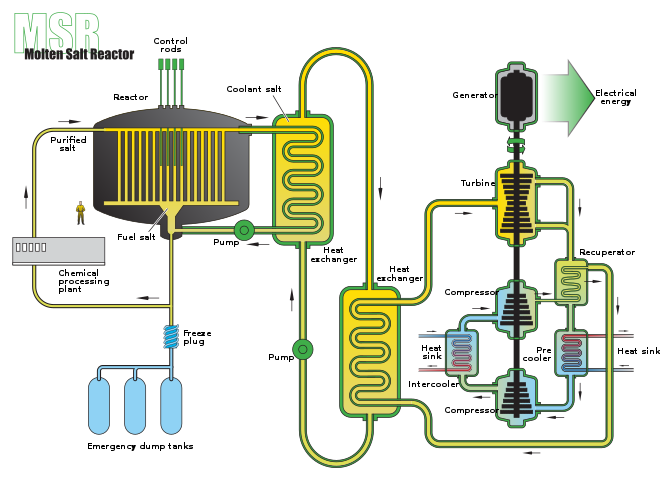
\includegraphics[height=2.8cm]{figures/msr}
          \hspace{1cm}
          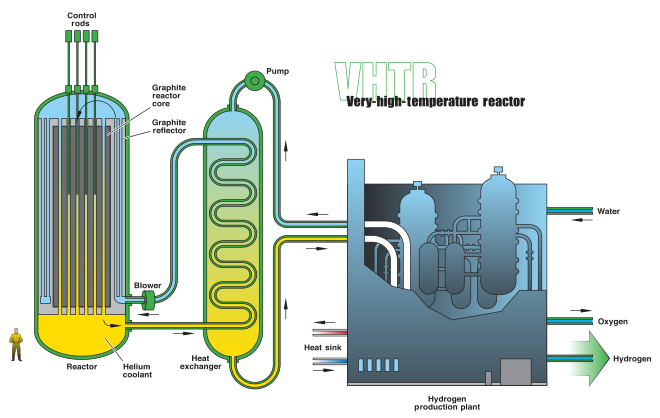
\includegraphics[height=2.8cm]{figures/vhtr}
      \end{figure}
    \end{itemize}
  \end{frame}
\begin{frame}
  \frametitle{Motivation}
  \begin{block}{Molten Salt Reactor (MSR) System}
    \begin{itemize}
      \item Produces fission power in circulating molten salt fuel mixture
      \item Molten Fluoride Salts have have chemical stability, low vapor pressure 
      at high temperatures, good heat transfer properties, resistance against 
      radiation damage, and inert to common structural materials
      \item Inherent system safety with fail-safe drainage, passive cooling, and 
      low inventory of volatile fission products in the fuel
    \end{itemize}
  \end{block}
  \begin{block}{Very High Temperature Reactor System (VHTR)}
    \begin{itemize}
      \item Tristructural Isotropic (TRISO) fuel withstands high burnup and 
      temperature
      \item High outlet temperature increases power conversion efficiency, reduces 
      waste heat generation, and enables high-temperature heat applications 
      such as hydrogen production
      \item Helium coolant's high 100 atm pressurization requires an expensive thick
      concrete reactor vessel
    \end{itemize}
  \end{block}
\end{frame}
\begin{frame}
  \frametitle{Motivation}
  \begin{itemize}
    \item \acrlong{FHR} concept combines the best aspects of \acrlong{MSR} and \acrlong{VHTR} technologies. 
      \acrshort{FHR} use high-temperature coated-particle fuel (similar to the \acrshortpl{VHTR}) 
      and a low-pressure liquid fluoride-salt coolant (similar to the \acrshortpl{MSR})
      \cite{forsberg_fluoride-salt-cooled_2012,facilitators_fluoride-salt-cooled_2013}.
  \end{itemize}
  \begin{block}{\acrfull{FHR} Benefits}
    \begin{itemize}
      \item FHR system has low operating pressure, thus does not require thick 
      concrete pressure vessel 
      \item Molten salt coolant has superior cooling and moderating properties 
      compared to helium coolant in VHTRs
      \item FHR system has large thermal margin enabled by molten salt coolant
      \item FHRs' TRISO particles' solid fuel cladding adds an extra barrier to 
      fission product release compared to MSRs with liquid fuel.
    \end{itemize}
  \end{block}
\end{frame}
\begin{frame}
  \frametitle{Motivation}
  \begin{block}{Advanced High Temperature Reactor Design}
    \begin{itemize}
      \item Design developed by Oak Ridge National Laboratory (ORNL)
      \item Prismatic FHR design with 252 hexagonal fuel assemblies consisting of 
      18 fuel planks arranged in 3 diamond-shaped sectors. 
    \end{itemize}
  \end{block}
  \begin{figure}[]
    \centering
    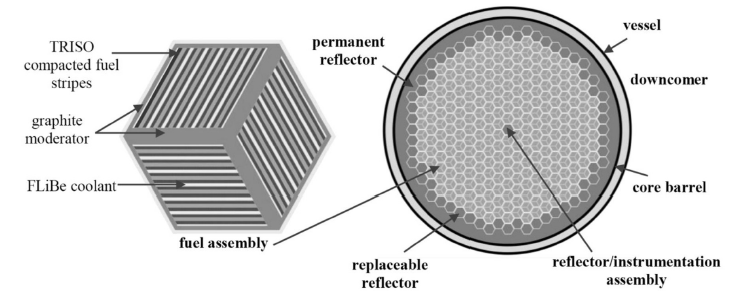
\includegraphics[width=0.8\linewidth]{../docs/figures/ahtr.png} 
    \caption{\acrlong{AHTR} fuel assembly (left) and core configuration (right) 
    reproduced from \cite{ramey_monte_2018}.}
    \label{fig:ahtr}
\end{figure}
\end{frame}

\begin{frame}
  \frametitle{Motivation}
  \begin{block}{Advanced High Temperature Reactor Design}
    \begin{itemize}
      \item Each fuel plank contains 2 fuel stripes that consists of a cubic 
      lattice of TRISO fuel particles
    \end{itemize}
  \end{block}
  \begin{figure}[]
    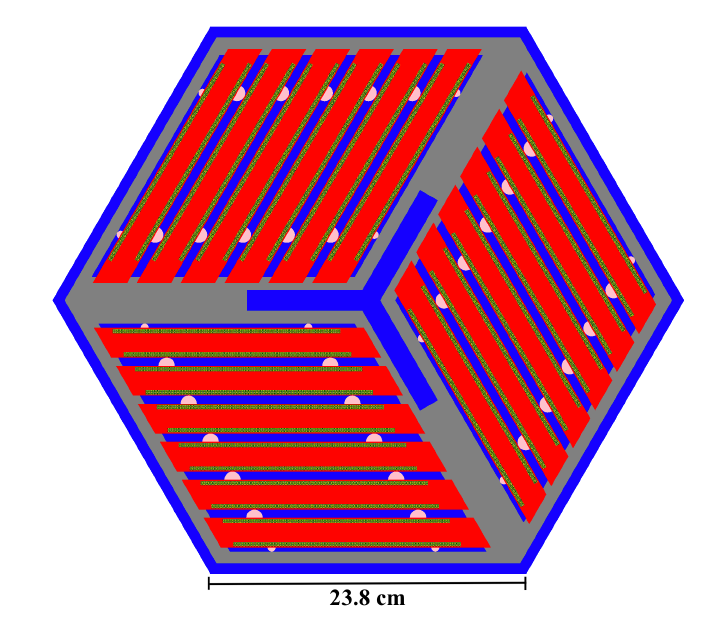
\includegraphics[width=0.5\linewidth]{figures/ahtr-assembly.png} 
    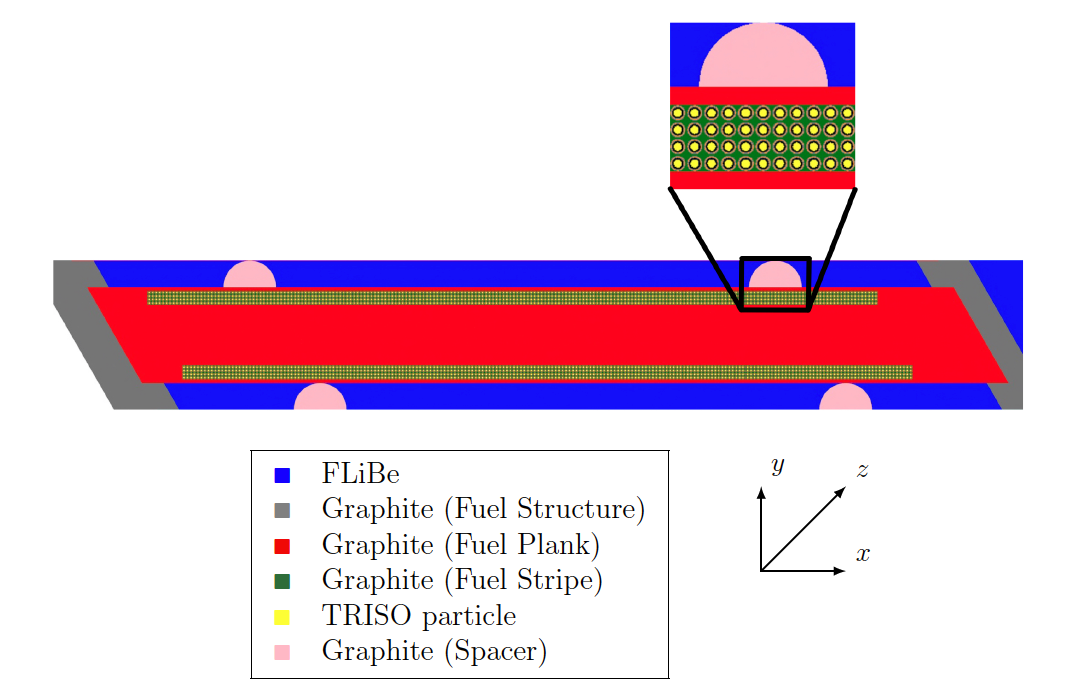
\includegraphics[width=0.5\linewidth]{figures/ahtr-plank.png} 
    \caption{\acrfull{AHTR} fuel assembly with 18 fuel plates arranged in 
    three diamond-shaped sectors, with a central Y-shaped and external channel 
    graphite structure.}
\end{figure}
\end{frame}

\begin{frame}
  \frametitle{Motivation}
  \begin{itemize}
    \item The AHTR's fuel geometry has triple heterogeneity resulting in
    complex reactor physics and significant modeling challenges
    \item To address and further understand the technical challenges for 
    AHTR modeling, in 2019 the OECD-NEA initiated a FHR benchmark exercise. Its objective 
    is to identify the applicability, accuracy, and practicality of the latest 
    methods and codes to assess the current state of the art of FHR simulation 
    and modeling. The benchmark also enables the cross-verification of software 
    and methods for the challenging AHTR geometry, which is especially useful 
    since applicable reactor physics experiments for code validation are scarce
  \end{itemize}
  \begin{figure}[]
    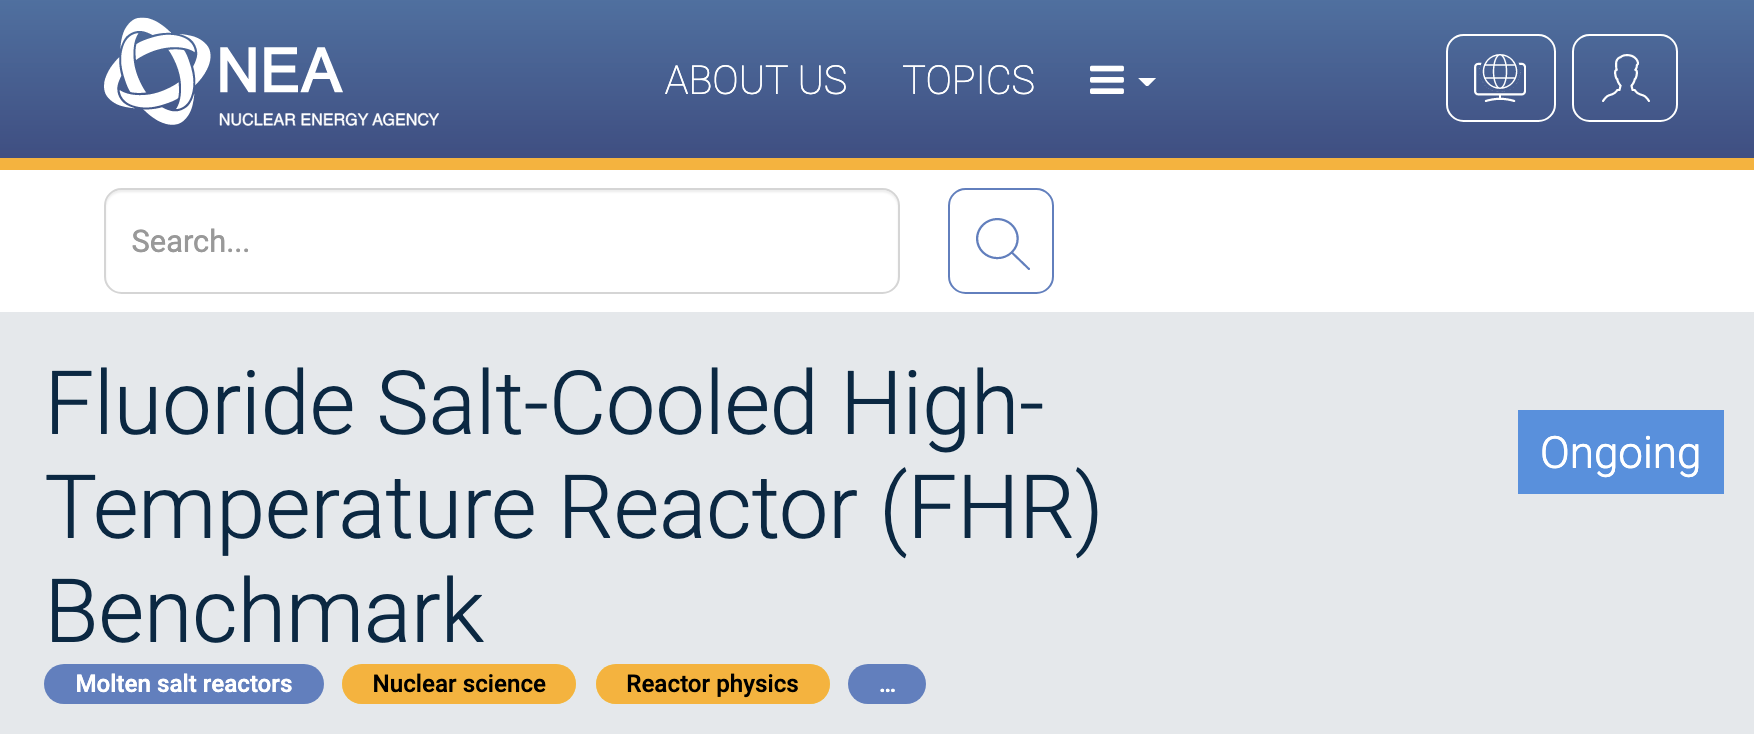
\includegraphics[width=0.7\linewidth]{figures/benchmark.png} 
    \caption{FHR Benchmark cite.}
\end{figure}
\end{frame}


\subsection{Objectives: AHTR Model Development}
\begin{frame}
  \frametitle{Research Objectives}
  \begin{block}{Technical Gap}
    \begin{itemize}
      \item The triple heterogeneity introduced by the geometrically complex 
      fuel assembly design makes accurate reactor physics simulations challenging. 
      Thus requiring a need to access accuracy of such analyses 
    \end{itemize}
  \end{block}
  \begin{block}{Proposed Work Component I: AHTR Model Development}
    \begin{itemize}
      \item I aim to further our understanding of the AHTR design's complexities 
      through neutronics and thermal-hydraulics modeling.
      \item I will participate in the OECD-NEA's FHR Benchmarking exercise with 
      OpenMC and Moltres
      \item Objectives 
      \begin{itemize}
        \item AHTR 2D and 3D assembly neutronics steady state and depletion models 
        with neutron transport software, OpenMC
        \item AHTR 2D fuel plank and assembly neutronics with thermal hydraulics 
        feedback using Moltres
      \end{itemize}
    \end{itemize}
  \end{block}
\end{frame}

\subsection{Background: Reactor optimization for non-conventional designs}
\begin{frame}
    \frametitle{3D Printing a Nuclear Reactor?}
    \begin{block}{Impact of Additive Manufacturing Technology Advancements on 
        Reactor Design Optimization}
        \begin{itemize}
            \item With further advancement of additive manufacturing technologies, a reactor 
            core could be 3D printed in the near future
            \item Leveraging additive manufacturing enables us to surpass classical 
            manufacturing constraints and optimize for arbitrary geometries and parameters 
            such as non-uniform channel shapes, and inhomogeneous fuel distribution 
            throughout the core
          \end{itemize}
    \end{block}
    \begin{figure}[]
      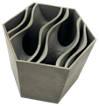
\includegraphics[width=0.2\linewidth]{figures/wavy-channels.png}
      \caption{Example of future reactor design with additively manufactured wavy 
      flow channels}
  \end{figure}
  \end{frame}

  \begin{frame}
    \frametitle{Evolutionary Algorithm Optimization}
    \begin{block}{Evolutionary Algorithms for Reactor Design Optimization}
    \begin{minipage}[c]{0.6\textwidth}
        \begin{itemize}
            \item We can leverage evolutionary algorithm optimization to 
            explore the large design space enabled by 3D printing to find global 
            optimal designs
            \item Evolutionary algorithms have proven successful in optimizing 
            multi-objective problems as they can find solutions at the global 
            optimum and take advantage of parallel systems
            \item Evolutionary algorithms imitate natural selection to evolve solutions 
            \end{itemize}
  \end{minipage}\hfill
  \begin{minipage}[c]{0.4\textwidth}
    \centering
    \begin{figure}
      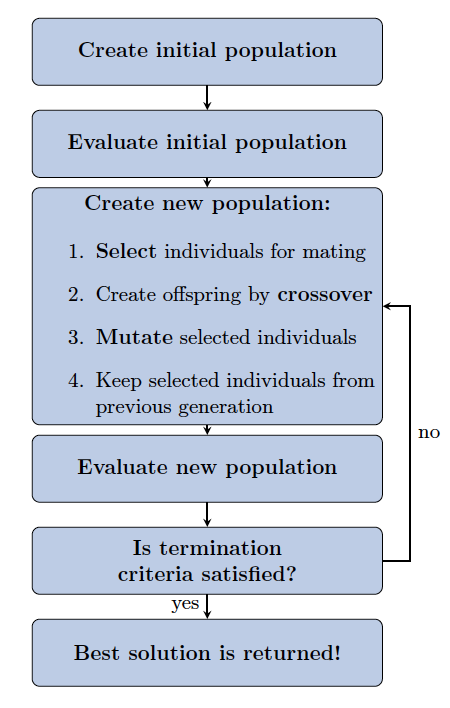
\includegraphics[width=0.8\linewidth]{figures/ea-flow.png} 
      \caption{Evolutionary algorithm flow \cite{renner_genetic_2003}. }
    \end{figure}
  \end{minipage}
  \end{block}
  \end{frame}
    

\subsection{Objectives: Reactor optimization for non-conventional designs}
\begin{frame}
    \frametitle{Research Objectives}
    \begin{block}{Technical Gap}
      \begin{itemize}
        \item Applying evolutionary algorithms to nuclear design problems is not new,
        however, evolutionary algorithm setup is highly customizable, A reactor 
        designer unfamiliar with evolutionary algorithms will have to go through 
        the cumbersome process of customizing a genetic algorithm for their
        needs and determine which operators and hyperparameters work best for their problem
      \end{itemize}
    \end{block}
    \begin{block}{Proposed Work Component II: Develop and demonstrate an evolutionary 
        algorithm optimization tool for multi-objective AHTR optimization of 
        non-conventional geometries and fuel distribution}
      \begin{itemize}
        \item Objectives
        \begin{itemize}
            \item Develop a tool that applies evolutionary algorithms with established 
            neutron transport and thermal hydraulics software to optimize reactor 
            design. The tool must be open-source, reproducible, effective, usable,
            and supports HPC parallelization. 
            \item Demonstrate successful implementation of the optimization tool 
            with OpenMC for single and multi-objective AHTR optimization
        \end{itemize}
        \end{itemize}
    \end{block}
  \end{frame}

\section{Methodology}
\subsection{FHR Benchmark Specifications}
\begin{frame}
    \frametitle{FHR Benchmark Specifications}
    \begin{itemize}
        \item Several organizations participate in the benchmark with various Monte Carlo
        and Deterministic neutronics software, such as Serpent \cite{leppanen_serpent_2014}, 
        OpenMC \cite{romano_openmc_2013}, and WIMS \cite{lindley_current_2017}. 
        \item UIUC participates in the benchmark with the OpenMC Monte Carlo code 
        \cite{romano_openmc_2013} using the ENDF/B-VII.1 material cross section library 
        \cite{chadwick_endf/b-vii.1_2011}.
        \item The benchmark will have three phases, starting from a single fuel assembly
        simulation without burnup (Phase I), gradually extending to full core depletion
        (Phase II) and multi-physics feedback (Phase III). 
    \end{itemize}
    \begin{table}
        \caption{\acrfull{OECD} \acrfull{NEA} \acrfull{FHR} Benchmark Phases 
        \cite{noauthor_fluoride_nodate}.}
        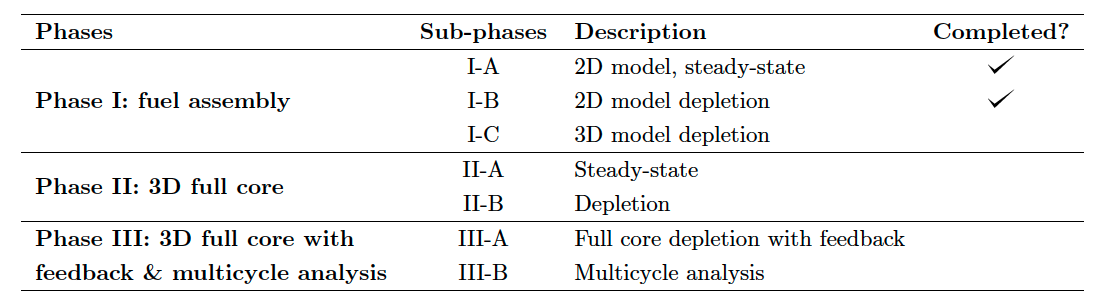
\includegraphics[width=0.8\linewidth]{figures/benchmark-phases.png} 
    \end{table}
\end{frame}

\begin{frame}
    \frametitle{FHR Benchmark Specifications}
    \begin{itemize}
        \item Only Phase I-A and I-B specifications have been released 
        \item Benchmark participants must produce the following results for 
        the 9 cases: $k_{eff}$, reactivity coefficients ($\beta_{eff}$, 
        $\alpha_D$, $\alpha_{T, FliBe}$, $\alpha_M$), fission source distribution, 
        neutron flux distribution, fuel assembly averaged neutron spectrum
    \end{itemize}
    \begin{table}
        \caption{Description of the \acrlong{FHR} benchmark Phase I-A cases 
        \cite{noauthor_fluoride_nodate}.}
        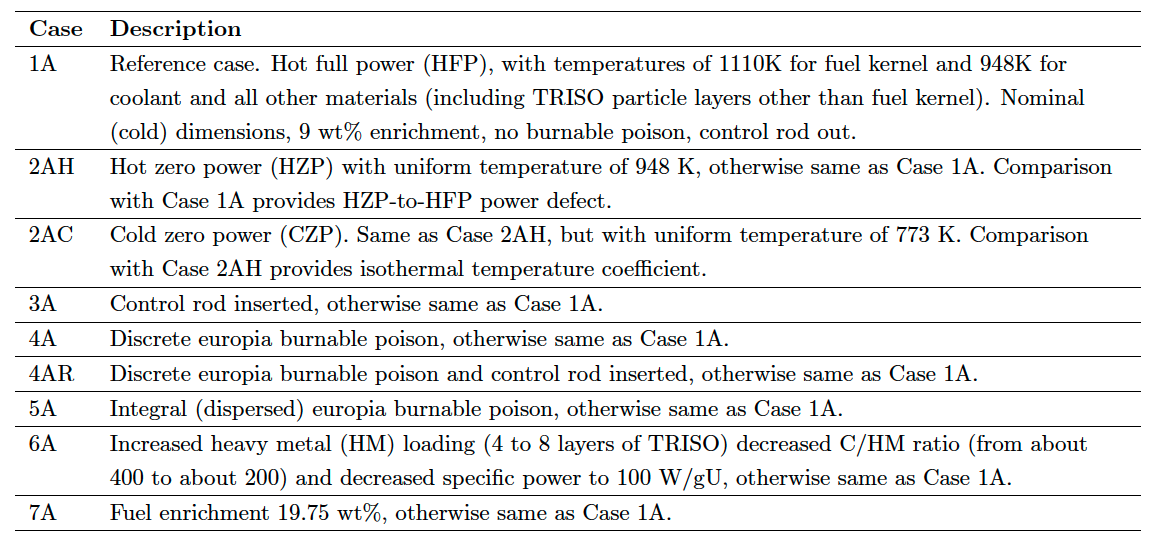
\includegraphics[width=0.8\linewidth]{figures/benchmark-cases.png} 
    \end{table}
\end{frame}
\subsection{Proposed Tool Design}
\begin{frame}
    \frametitle{Optimization Tool's Design Goals}
    \begin{minipage}[c]{0.45\textwidth}
    \begin{itemize}
        %\item ROLLO (Reactor evOLutionary aLgorithm Optimizer) is a Python package 
        %that applies evolutionary algorithms to optimize nuclear reactor design
        \item The tool couples an evolutionary algorithm driver, Distributed 
        Evolutionary Algorithms in Python (DEAP), with 
        nuclear software, such as neutron transport OpenMC and thermal-hydraulics 
        Moltres codes
        \item Design Goals: effective, flexible, open-source, parallel,
        reproducible
    \end{itemize}
    \end{minipage}\hfill
    \begin{minipage}[c]{0.55\textwidth}
        \centering
        \begin{figure}
            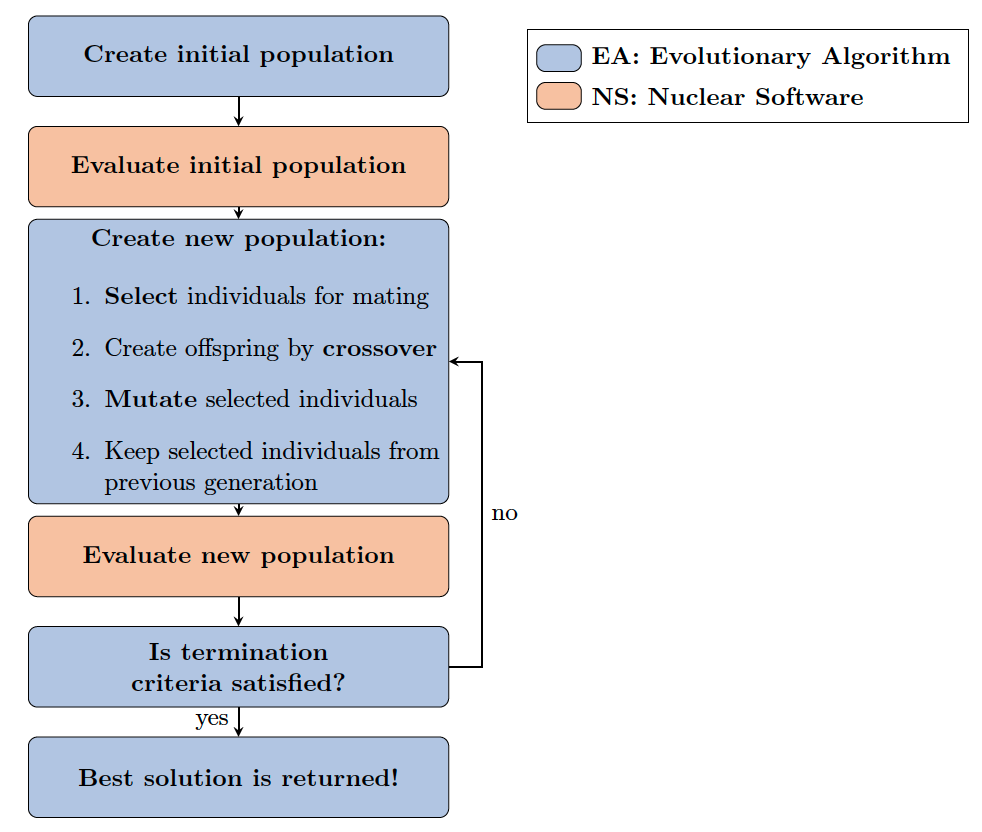
\includegraphics[width=\linewidth]{figures/rollo-flow.png} 
            \caption{Optimization tool's flow.}
        \end{figure}
    \end{minipage}
    %\begin{block}{ROLLO Design Goals}
    %    \begin{itemize}
    %        \item Effective: good documentation, well tested, version controlled 
    %        on Github 
    %        \item Flexible: user can vary any imaginable parameter because
    %       ROLLO uses a templating method to edit the input file of the coupled software.
    %        \item Open-source: utilizes only open-source dependencies 
    %        \item Parallel: toggle to enable parallelization on local and HPCs
    %        \item Reproducible: Data from every ROLLO run saves into a unique, 
    %        pickled file (pickle is a Python module that serializes Python 
    %        objects), and all results from this work are available on Github.
    %    \end{itemize}
    %\end{block}
\end{frame}

\section{Component I: Proposed Work and Preliminary Results}
\subsection{Proposed Work's Component I: Progress Chart}
\begin{frame}
    \frametitle{Proposed Work's Component 1 Progress}
    \begin{itemize}
        \item Proposed Work's Component I: AHTR Model Development for the FHR Benchmark
    \end{itemize}
    \vspace{-0.8cm}
    \begin{figure}[]
        \centering
        \resizebox{\textwidth}{!}{
        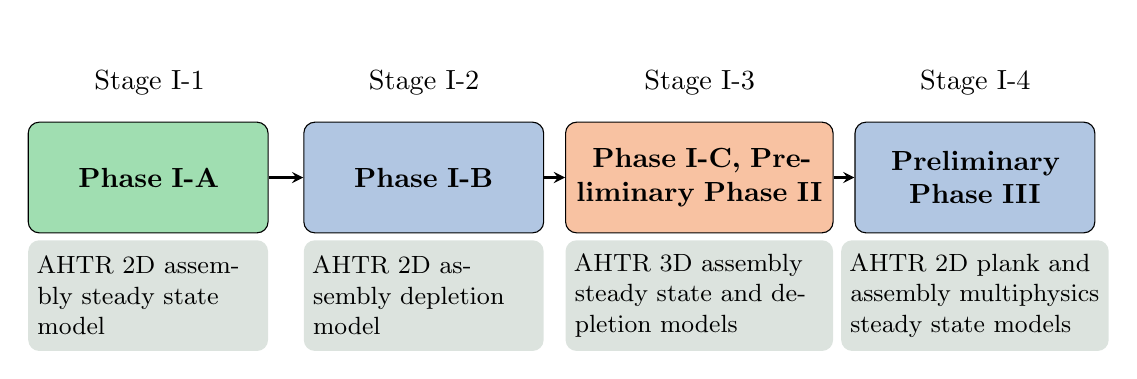
\begin{tikzpicture}[node distance=3.5cm,auto,>=latex']
            \node [gblock] (a) {\textbf{Phase I-A}};
            \node [bblock] (b) [right of=a] {\textbf{Phase I-B}};
            \node [oblock] (c) [right of=b] {\textbf{Phase I-C, Preliminary Phase II}};
            \node [bblock] (d) [right of=c] {\textbf{Preliminary Phase III}};
            \node [noblock] (e) [above of=a, yshift=-2.3cm] {Stage I-1};
            \node [noblock] (e) [above of=b, yshift=-2.3cm] {Stage I-2};
            \node [noblock] (e) [above of=c, yshift=-2.3cm] {Stage I-3};
            \node [noblock] (e) [above of=d, yshift=-2.3cm] {Stage I-4};
            \node [greyblock] (e) [below of=a, yshift= 2cm, font=\small] {AHTR 2D assembly steady state model};
            \node [greyblock] (e) [below of=b, yshift= 2cm, font=\small] {AHTR 2D assembly depletion model};
            \node [lgreyblock] (e) [below of=c, yshift= 2cm, font=\small] {AHTR 3D assembly steady state and depletion models};
            \node [lgreyblock] (e) [below of=d, yshift= 2cm, font=\small] {AHTR 2D plank and assembly multiphysics steady state models};
            \draw [arrow] (a) -- (b);
            \draw [arrow] (b) -- (c);
            \draw [arrow] (c) -- (d);
        \end{tikzpicture}}
    \end{figure}
    \begin{figure}
        \resizebox{0.25\textwidth}{!}{
            \fbox{\begin{tabular}{ll}
                \textcolor{illinigreen}{$\blacksquare$} & Completed \\
                \textcolor{illiniblue}{$\blacksquare$} & In Progress \\
                \textcolor{illiniorange}{$\blacksquare$} & Planned \\
                \end{tabular}}}
    \end{figure}
\end{frame}
\subsection{Stage I-1: FHR Benchmark Phase I-A (Completed)}
\begin{frame}
    \frametitle{Completed Stage I-1: FHR Benchmark Phase I-A Results}
    \begin{itemize}
        \item FHR Benchmark Phase I-A: 2D assembly steady state model
        \item In a recently submitted ANS M$\&$C 2021 conference paper 
        (which I am a co-author on), 
        Petrovic et al. \cite{petrovic_preliminary_2021} compared FHR benchmark 
        participants' Phase I-A $k_{eff}$ results.  
        We reported that the standard deviation between participants for each case 
        was in the 231 to 514 pcm range, acceptable and notably close given a blind 
        benchmark, assuring that \gls{UIUC}'s Phase I-A results are acceptable and 
        in agreement with other benchmark participants 
    \end{itemize}
    \begin{figure}[]
        \begin{minipage}[c]{0.5\textwidth}
        \centering
        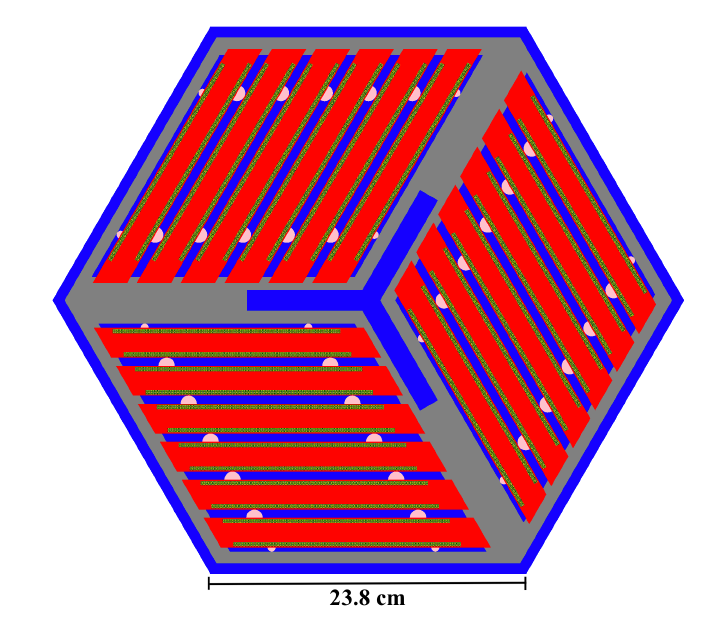
\includegraphics[width=0.75\linewidth]{figures/ahtr-assembly.png} 
        \end{minipage}\hfill
        \begin{minipage}[c]{0.5\textwidth}
        \caption{\acrfull{AHTR} fuel assembly with 18 fuel plates arranged in 
        three diamond-shaped sectors, with a central Y-shaped and external channel 
        graphite structure.}
        \end{minipage}
    \end{figure}
\end{frame}

\begin{frame}
    \frametitle{Completed Stage I-1: FHR Benchmark Phase I-A Results}
    \begin{table}
        \caption{\acrlong{UIUC}'s \acrlong{FHR} Benchmark Phase I-A results 
        \cite{chee_arfcfhr-benchmark_2021}.}
        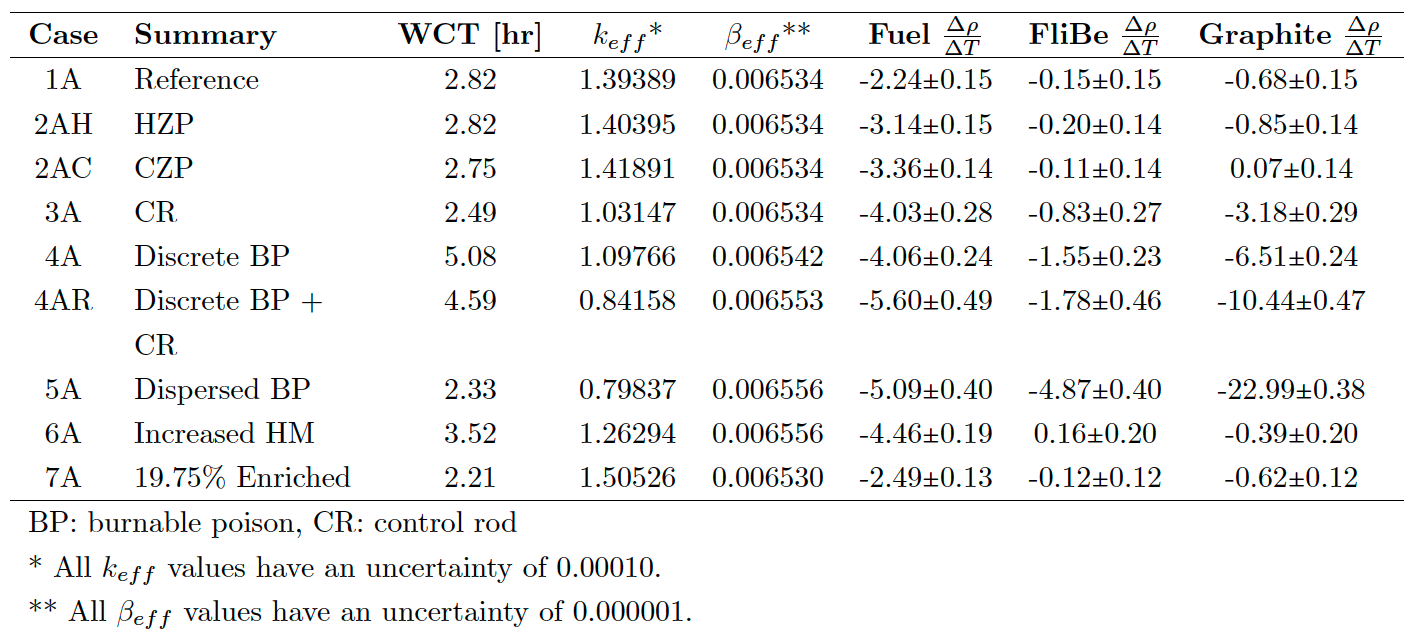
\includegraphics[width=\linewidth]{figures/benchmark-coeff-results.png} 
    \end{table}
\end{frame}

\begin{frame}
    \frametitle{Completed Stage I-1: FHR Benchmark Phase I-A Results}
    \begin{figure}[]
        \centering
        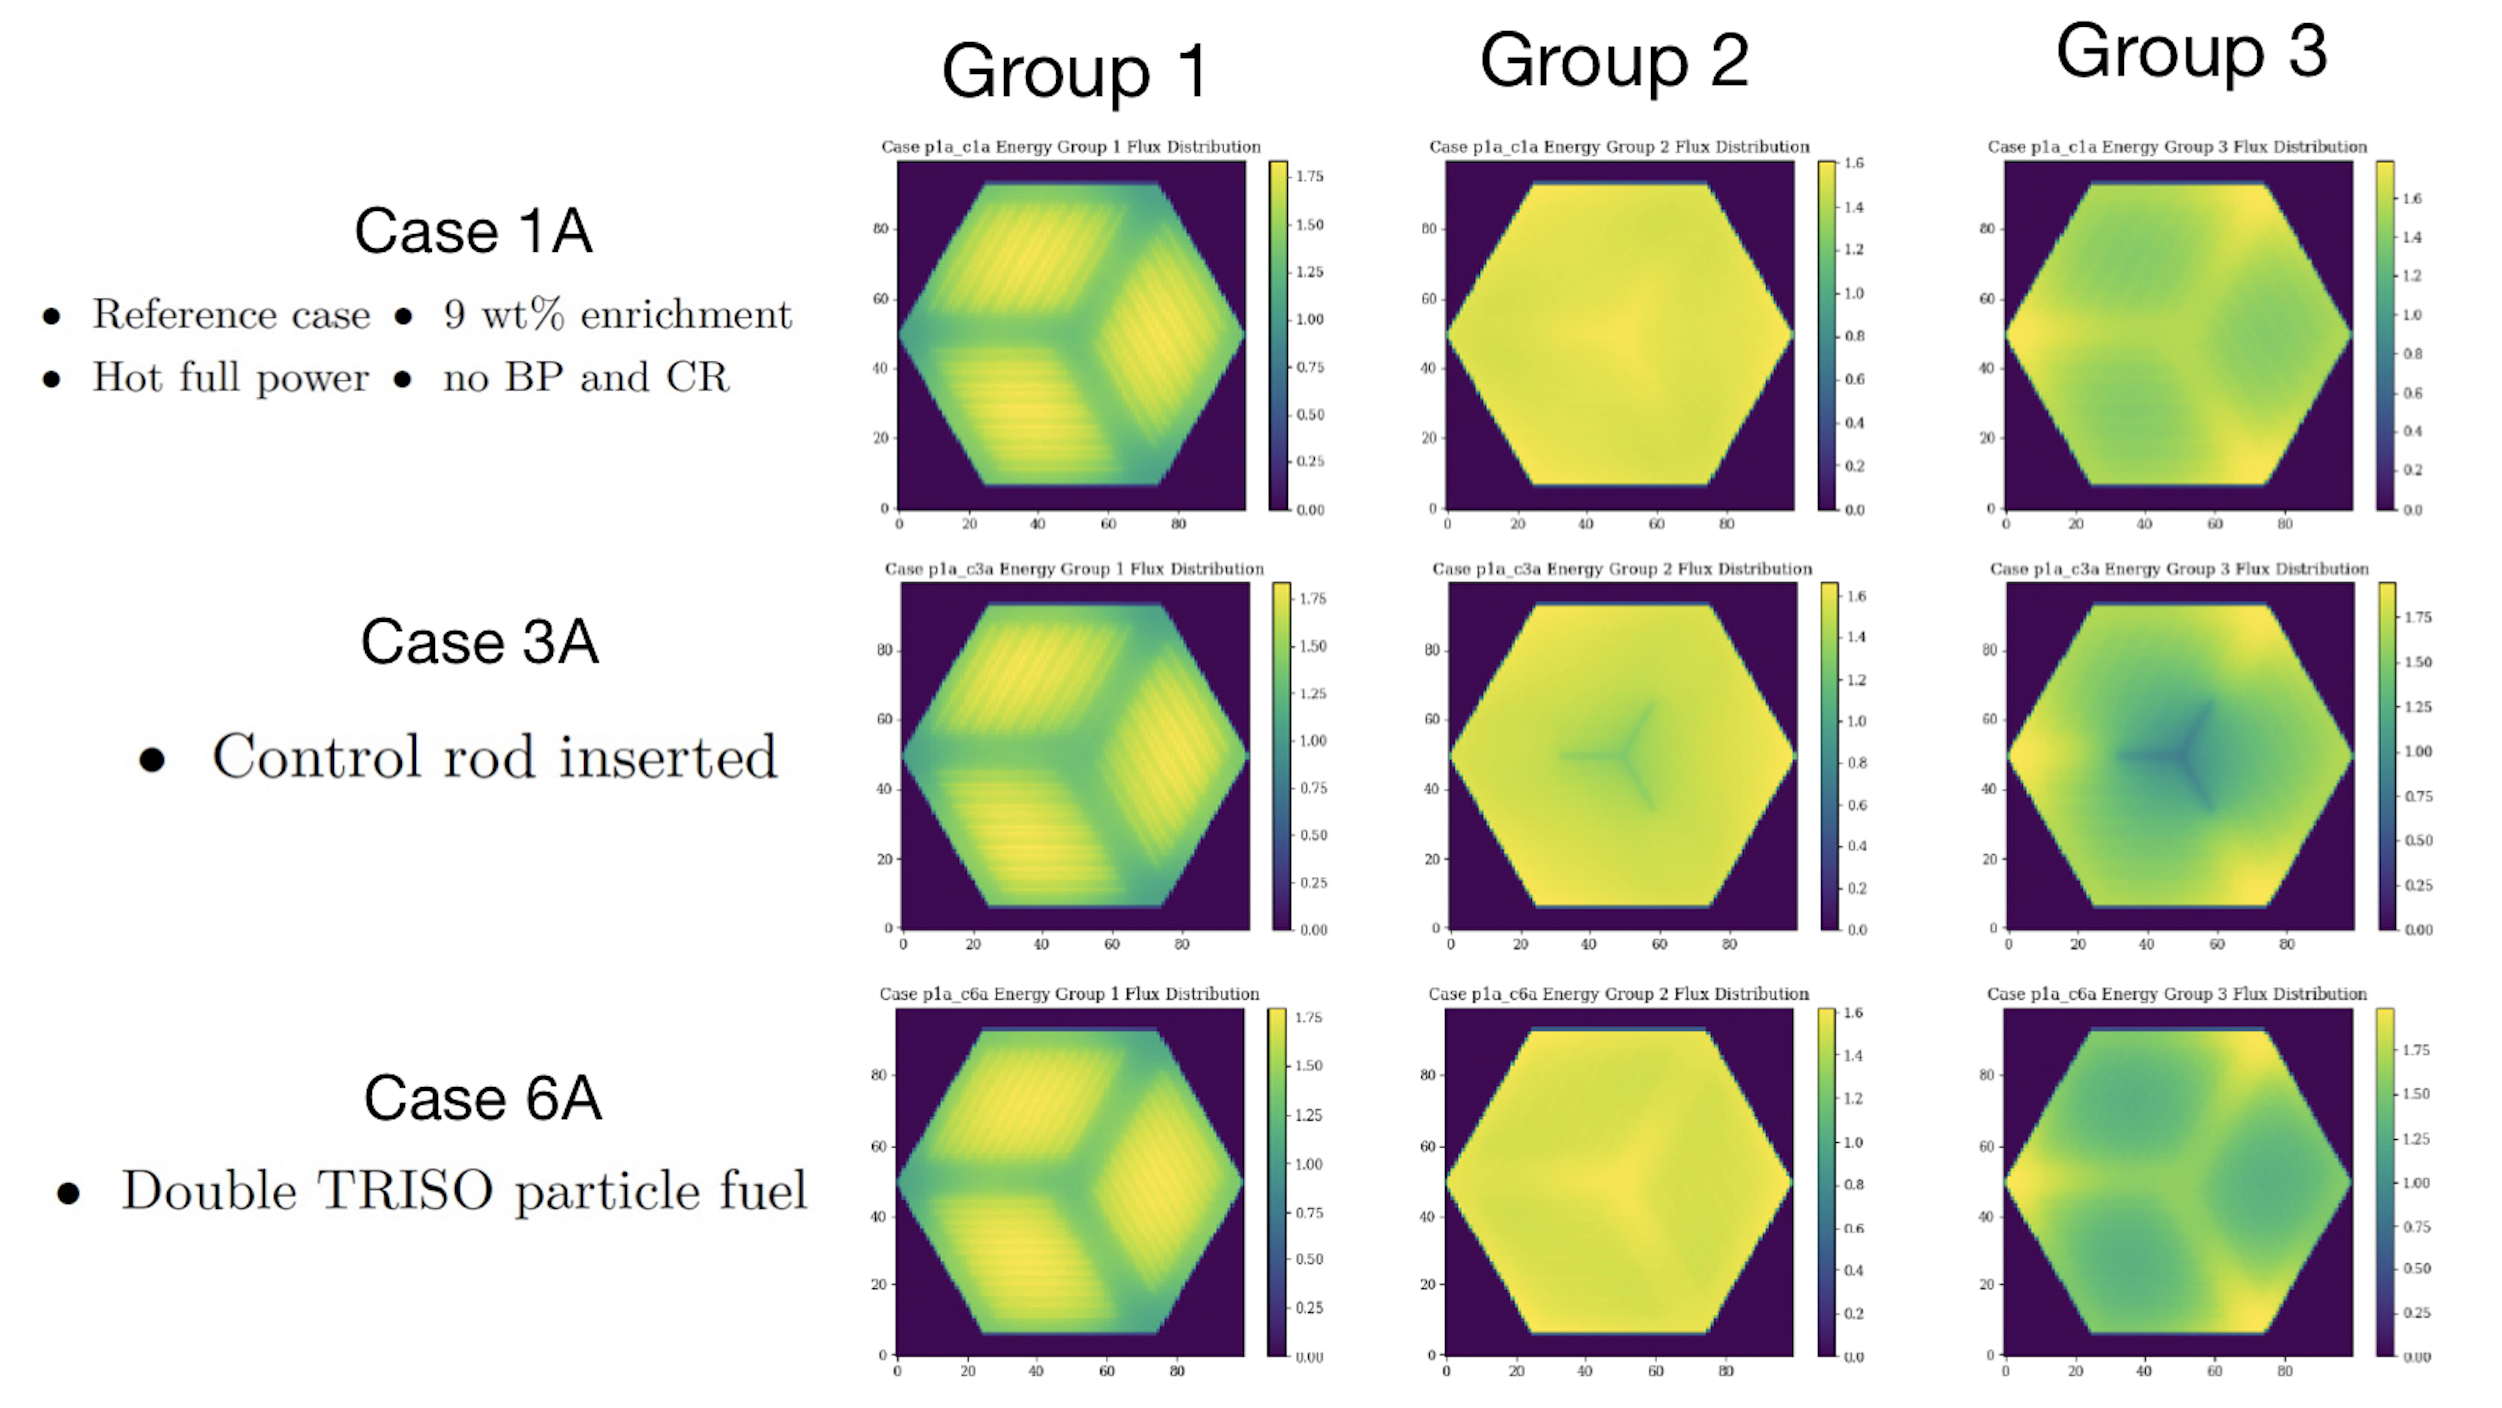
\includegraphics[width=0.6\linewidth]{figures/phase1a-e.png} 
        \caption{UIUC results: FHR Benchmark neutron flux 
        distribution in 100 $\times$ 100 mesh for three coarse energy groups: Case 
        1A (above), Case 3A (middle), Case 6A (below). Energy group 1: $E > 0.1$ MeV, 
        Energy group 2: $3 \times 10^{-6} < E < 0.1$ MeV, Energy group 3: $E < 3 \times 10^{-6}$ MeV. }
    \end{figure}
\end{frame}
\subsection{Stage I-2: FHR Benchmark Phase I-B (In Progress)}
\begin{frame}
    \frametitle{In Progress Stage I-2: FHR Benchmark Phase I-B Results}
    \begin{itemize}
        \item FHR Benchmark Phase I-B: 2D assembly depletion model
        \item Benchmark participants are working on resolving differences in 
        these results
    \end{itemize}
    \vspace{-0.2cm}
    \begin{figure}[]
        \centering
        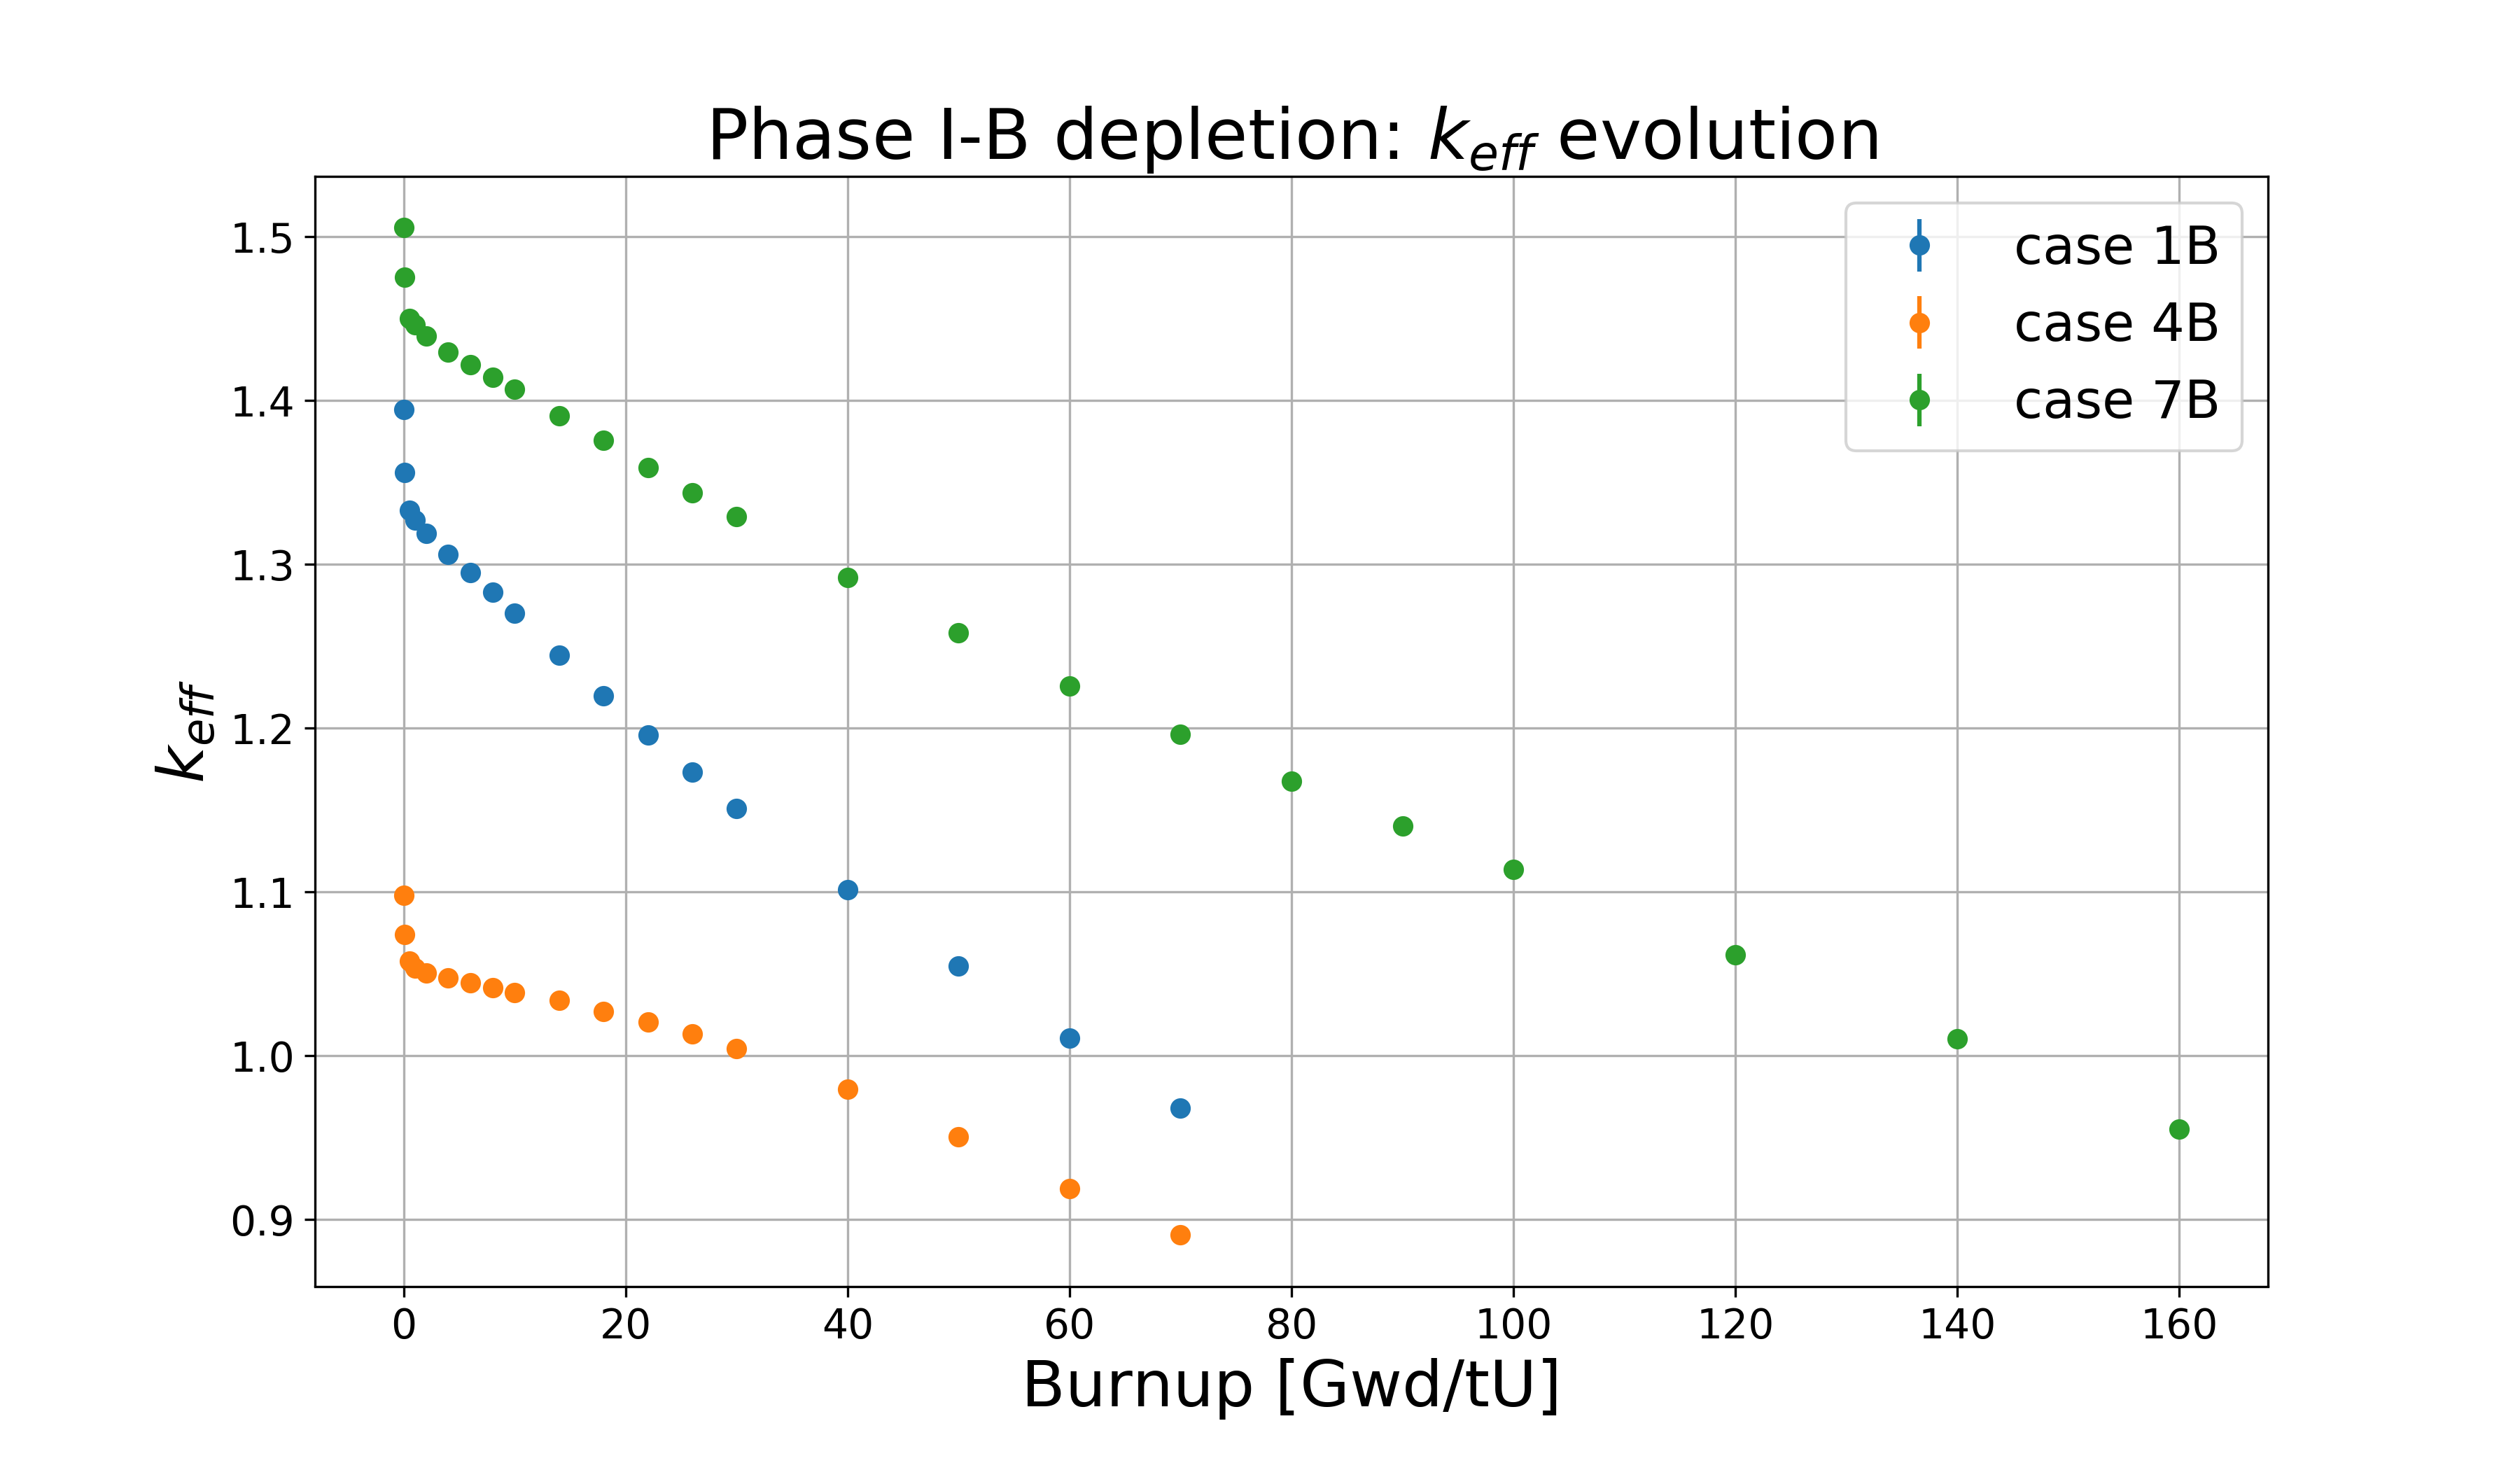
\includegraphics[width=0.75\linewidth]{../docs/figures/phase1b_keff.png} 
        \caption{UIUC results: FHR Benchmark Phase I-B depletion 
        $k_{eff}$ evolution for Cases 1B, 4B, and 7B. Case 1B is the reference case, 
        Case 4B is the discrete \acrlong{BP} case, and Case 7B is the 19.75$\%$ 
        enrichment case. Error bars are included but are barely visible due to the 
        low $\sim$40pcm uncertainty.}
    \end{figure}
\end{frame}
\subsection{Stage I-3: FHR Benchmark Phase I-C and II (Planned)}
\begin{frame}
    \frametitle{Planned Stage 1-3: FHR Benchmark Phase I-C Planned Work}
        \begin{itemize}
            \item FHR benchmark's Phase I-C extends the 2D assembly model from 
            Phases I-A and I-B into a 3D assembly model
            \item Benchmark organizers will release the Phase I-C detailed 
            specifications and required results in late 2021
            \item When the specifications are released, I will contribute Phase I-C
            results to the benchmark
        \end{itemize}
    %\begin{block}{Preliminary Phase II}
    %    \begin{itemize}
    %        \item FHR Benchmark Phase II: 3D full core steady state and depletion 
    %        models 
    %        \item For preliminary work towards Phase II, I will expand the AHTR model 
    %        from assembly to full core 
    %    \end{itemize}
    %\end{block}
\end{frame}
\subsection{Stage I-4: FHR Benchmark III (Planned)}
\begin{frame}
    \frametitle{In Progress Stage I-4: FHR Benchmark Phase III Goals}
    \begin{itemize}
        \item FHR Benchmark Phase III: 3D full core with feedback and multicycle 
        analysis
        \item I will use the open-source MSR simulation tool, Moltres, to conduct
        AHTR multiphysics simulations for fuel slab geometry and one-third 
        fuel assembly geometry. 
        \item Moltres, an application built atop the 
        \gls{MOOSE} parallel finite element framework \cite{gaston_moose:_2009}, 
        contains physics kernels and boundary conditions to solve arbitrary-group 
        deterministic neutron diffusion and thermal-hydraulics \glspl{PDE} 
        simultaneously on a single mesh \cite{lindsay_introduction_2018,park_advancement_2020}. 
        \item AHTR Moltres simulations will capture thermal feedback effects, 
        absent from the purely neutronics OpenMC simulations.  
    \end{itemize}
\end{frame}

\begin{frame}
    \frametitle{In Progress Stage I-4: FHR Benchmark Phase III Preliminary Work}
    \begin{itemize}
        \item To run Moltres simulations, the user provides group constant data from a neutron 
        transport solver, such as OpenMC, for the Moltres multigroup neutron diffusion 
        calculations and a mesh file representing the reactor geometry. 
        A TRISO-level fidelity mesh file is impractical and will result in an extremely 
        long Moltres runtime. 
        \item For successful AHTR Moltres simulation, I must establish 
        suitable spatial and energy homogenization that preserves accuracy while 
        maintaining an acceptable runtime.
    \end{itemize}
\begin{block}{Spatial Homogenization}
    \begin{itemize}
        \item I discretized the fuel slab into 13 cells: FLiBe, left graphite, right graphite, 
    and ten fuel cells (each cell has a different packing fraction)
    \end{itemize}
    \vspace{-0.3cm}
    \begin{figure}[]
        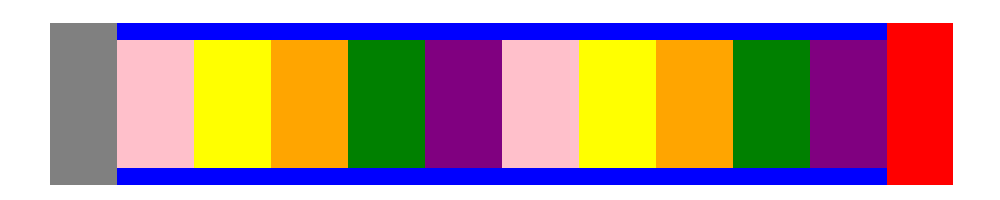
\includegraphics[width=0.6\linewidth]{../docs/figures/straightened_slab_mg.png}
        \caption{Straightened AHTR fuel slab spatially discretized into 
        13 \textit{cells} for OpenMC multigroup calculation.}
    \end{figure}
\end{block}
\end{frame}

\begin{frame}
    \frametitle{In Progress Stage I-4: FHR Benchmark Phase III Preliminary Work}
    \begin{block}{Energy Homogenization}
        \begin{itemize}
            \item I used the four group energy structure derived by Gentry et al. 
            \cite{gentry_development_2016} for AHTR geometries. 
        \end{itemize}
        \vspace{-0.4cm}
        \begin{table}[]
            \centering
            \begin{minipage}[c]{0.5\textwidth}
                \centering
                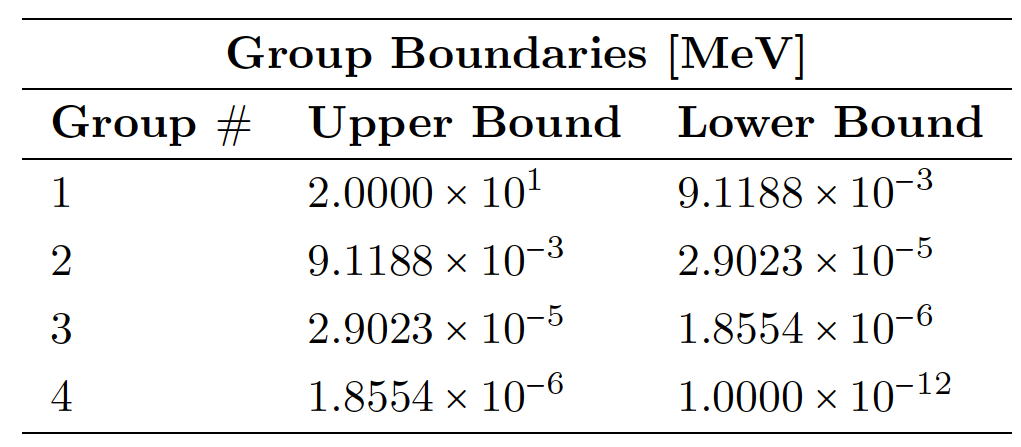
\includegraphics[width=0.6\linewidth]{figures/ahtr-energy-discr.png}
            \end{minipage}\hfill
            \begin{minipage}[c]{0.5\textwidth}
            \caption{4-group energy structures for AHTR geometry 
            derived by \cite{gentry_development_2016}.}
        \end{minipage}
        \end{table}
    \end{block}
    \vspace{-0.3cm}
    \begin{block}{Simulation Comparison: Continuous energy vs spatial 
        and energy homogenized}
        \begin{itemize}
            \item The 26pcm difference between $k_{eff}$ values is within both uncertainty values, 
            assuring that the spatial and energy homogenization used is suitable for generating 
            group constants for Moltres. 
        \end{itemize}
        \vspace{-0.3cm}
        \begin{table}[]
            \centering
            \begin{minipage}[c]{0.6\textwidth}
                \centering
                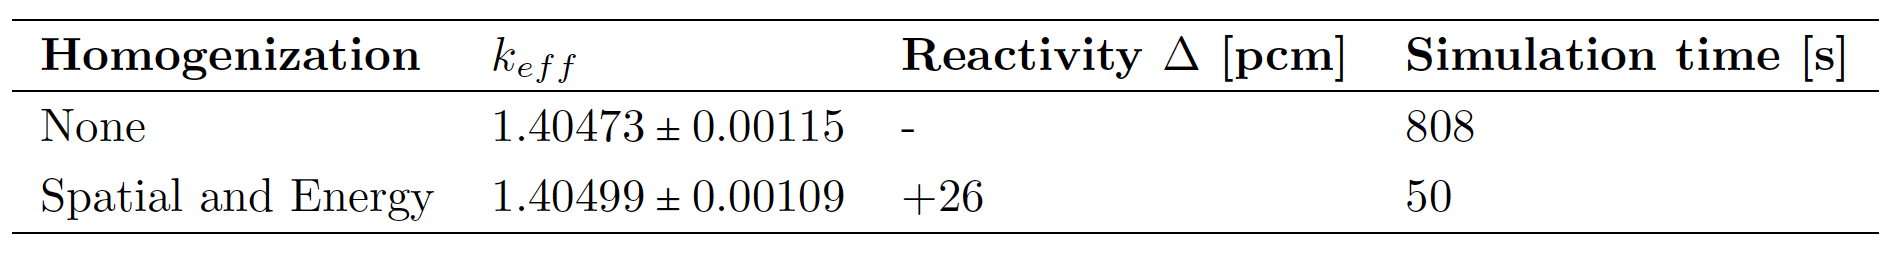
\includegraphics[width=0.8\linewidth]{figures/ahtr-homogenization.png}
            \end{minipage}\hfill
            \begin{minipage}[c]{0.4\textwidth}
            \caption{
            Both simulations were run on one BlueWaters XE Node, with 80 active cycles, 
            20 inactive cycles, and 8000 particles.}
        \end{minipage}
        \end{table}
    \end{block}
\end{frame}

\section{Component II: Proposed Work and Preliminary Results}
\subsection{Proposed Work's Component II: Progress Chart}
\begin{frame}
    \frametitle{Proposed Work's Component 2 Progress}
    \begin{itemize}
        \item Proposed Work's Component II: ROLLO Development and AHTR Optimization 
        Demonstration
    \end{itemize}
    \vspace{-0.8cm}
    \begin{figure}[]
        \centering
        \resizebox{\textwidth}{!}{
        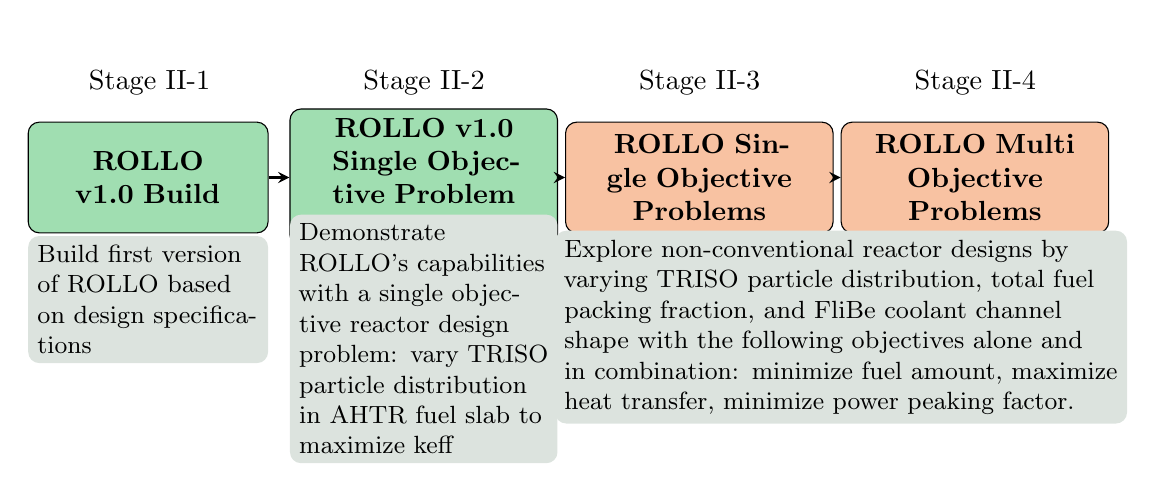
\begin{tikzpicture}[node distance=1.2cm,auto,>=latex']
            \node [gblock] (a) {\textbf{ROLLO v1.0 Build}};
            \node [lgblock] (b) [right of=a, xshift=2.3cm] 
            {\textbf{ROLLO v1.0 Single Objective Problem Demonstration}};
            \node [oblock] (c) [right of=b, xshift=2.3cm] 
            {\textbf{ROLLO Single Objective Problems}};
            \node [oblock] (d) [right of=c, xshift=2.3cm] 
            {\textbf{ROLLO Multi Objective Problems}};
            \node [noblock] (e) [above of=a] {Stage II-1};
            \node [noblock] (e) [above of=b] {Stage II-2};
            \node [noblock] (e) [above of=c] {Stage II-3};
            \node [noblock] (e) [above of=d] {Stage II-4};
            \node [greyblock] (e) [below of=a, yshift= -0.35cm, font=\small] 
            {Build first version of ROLLO based on design specifications};
            \node [lgreyblock] (e) [below of=b, yshift= -0.85cm, font=\small] 
            {Demonstrate ROLLO's capabilities with a single objective reactor 
            design problem: vary TRISO particle distribution in AHTR fuel slab 
            to maximize keff};
            \node [llgreyblock] (e) [below of=c, xshift=1.8cm, yshift= -0.7cm, font=\small] 
            {Explore non-conventional reactor designs by varying TRISO particle 
            distribution, total fuel packing fraction, and FliBe coolant channel
            shape with the following objectives alone and in combination: 
            minimize fuel amount, maximize heat transfer, minimize power peaking 
            factor.};
            \draw [arrow] (a) -- (b);
            \draw [arrow] (b) -- (c);
            \draw [arrow] (c) -- (d);
        \end{tikzpicture}}
    \end{figure}
\begin{figure}
    \resizebox{0.25\textwidth}{!}{
        \fbox{\begin{tabular}{ll}
            \textcolor{illinigreen}{$\blacksquare$} & Completed \\
            \textcolor{illiniblue}{$\blacksquare$} & In Progress \\
            \textcolor{illiniorange}{$\blacksquare$} & Planned \\
            \end{tabular}}}
\end{figure}
\end{frame}
\subsection{Stage II-1: ROLLO v1.0 Build (Completed)}
\begin{frame}
    \frametitle{Completed Stage 2-1: ROLLO v1.0 Build}
    \begin{figure}
        \centering
        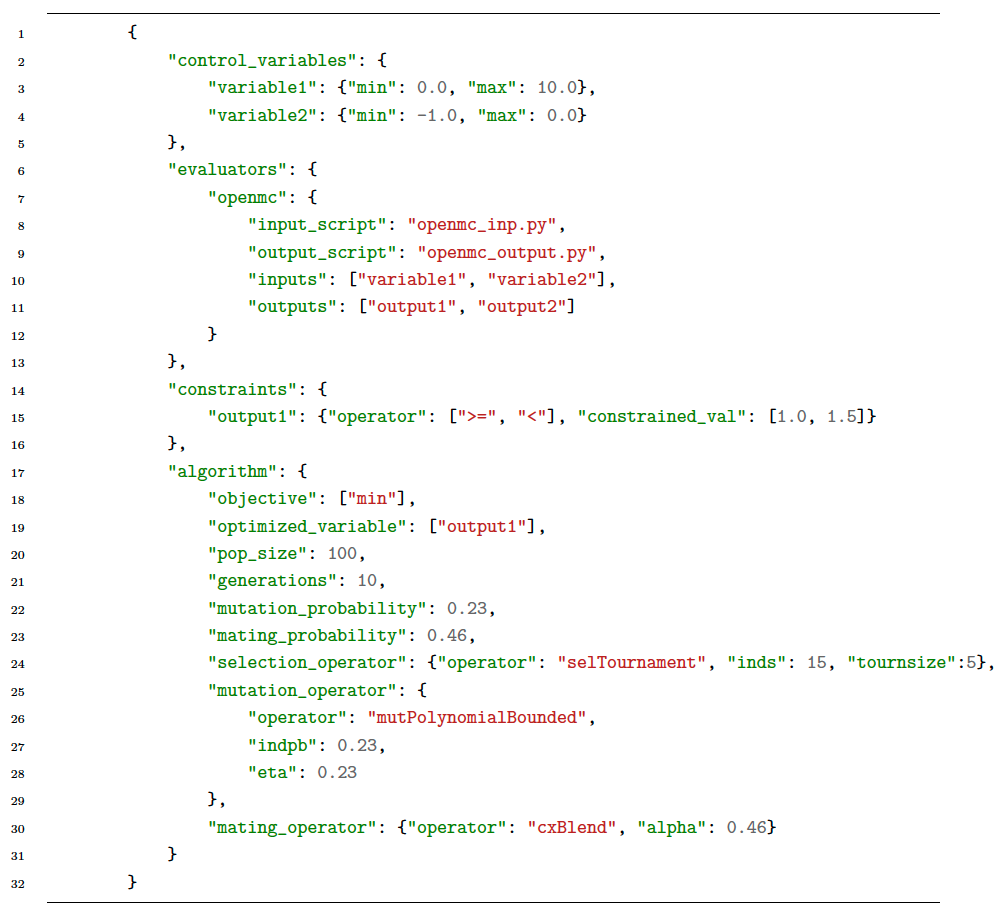
\includegraphics[width=0.65\linewidth]{figures/rollo-json-input.png} 
        \caption{ROLLO sample JSON input file.}
    \end{figure}
\end{frame}

\begin{frame}
    \frametitle{ROLLO Class Architecture}
    \begin{figure}
        \centering
        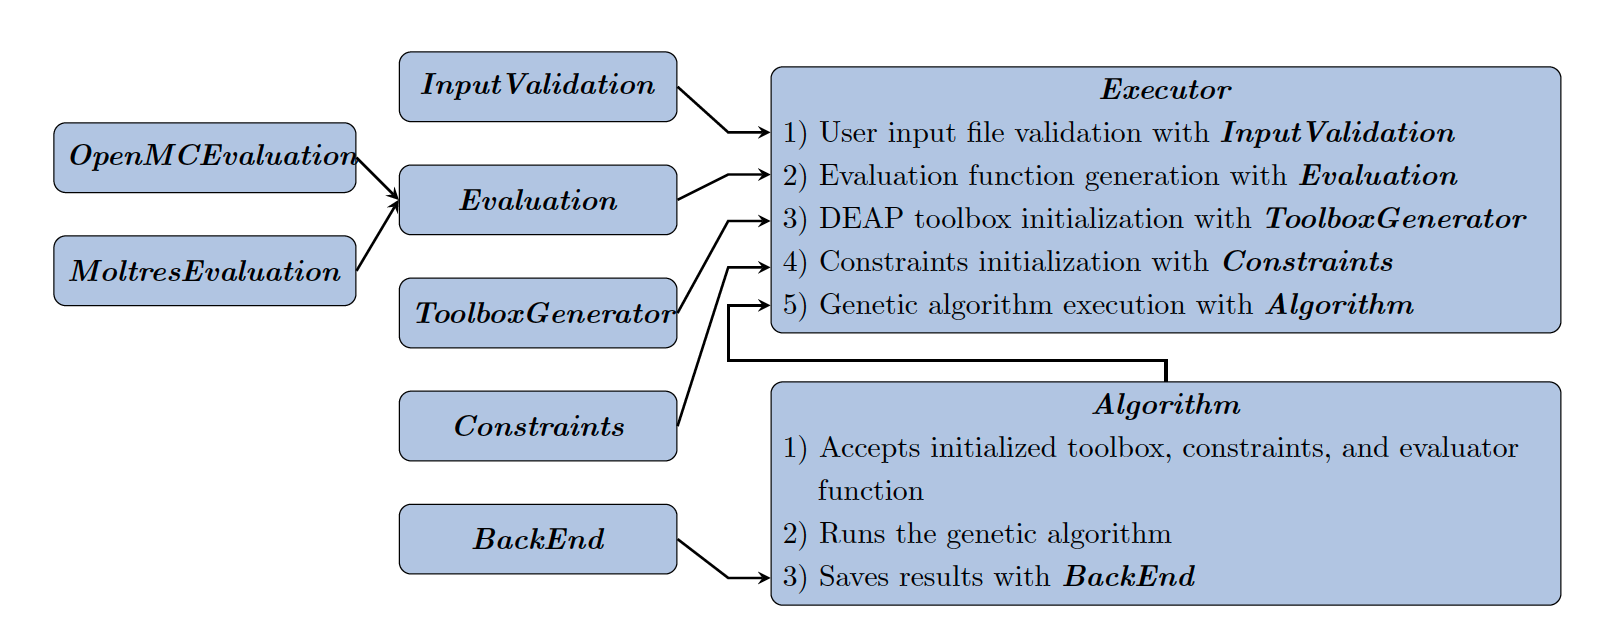
\includegraphics[width=\linewidth]{figures/rollo-architecture.png} 
        \caption{Visualization of ROLLO architecture.}
    \end{figure}
\end{frame}
\subsection{Stage II-2: ROLLO v1.0 Demonstration (Completed)}
\begin{frame}
    \frametitle{Completed Stage II-2: ROLLO v1.0 Demonstration}
    \begin{itemize}
        \item I demonstrate ROLLO's capabilities with a single objective design 
        problem: maximize $k_{eff}$ by varying TRISO particle distribution in an 
        AHTR fuel slab while keeping total packing fraction constant
        \item I divided the slab into ten cells along the x-axis between the FliBe and 
        graphite buffers, resulting in ten cells. A sine distribution governs the 
        TRISO particle packing fraction's distribution across cells:
    \end{itemize}
    \small
    \begin{align*}
        PF(x) &= \left(a\cdot sin(b\cdot x + c) + 2\right) \cdot NF\\
        \intertext{where}
        PF &= \mbox{packing fraction } [-] \nonumber \\ 
        a &= \mbox{amplitude, peak deviation of the function from zero } [-] \nonumber \\
        b &= \mbox{angular frequency, rate of change of the function argument } [\frac{radians}{cm}] \nonumber \\
        c &= \mbox{phase, the position in its cycle the oscillation is at t = 0 } [radians]\nonumber \\
        x &= \mbox{midpoint value for each cell } [cm]\nonumber \\
        NF &= \mbox{Normalization factor } [-]\nonumber
    \end{align*}
\end{frame}

\begin{frame}
    \frametitle{Completed Stage II-2: Prolem Defintion}
    \begin{figure}[]
        \centering
        \makebox[\textwidth][c]{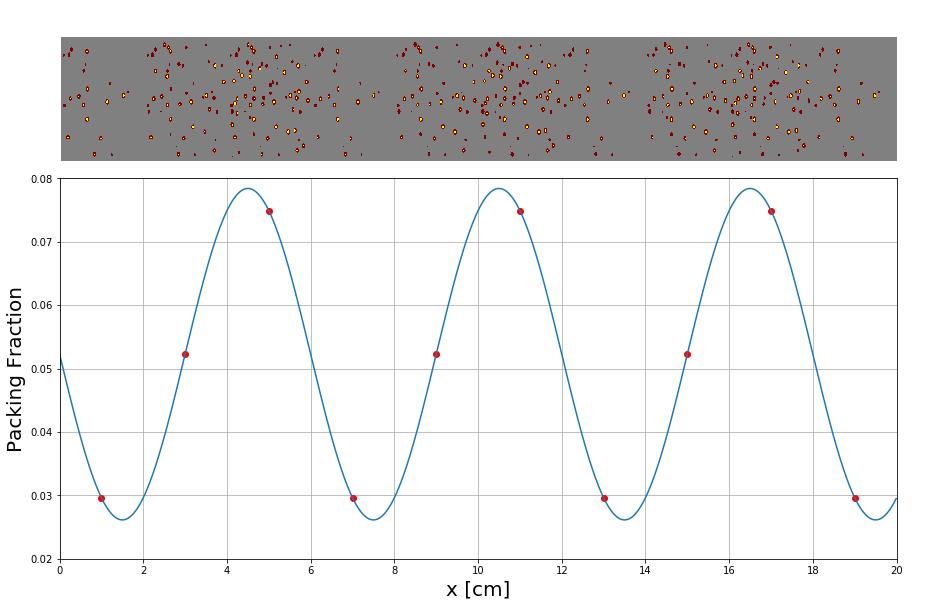
\includegraphics[width=0.9\linewidth]{../docs/figures/triso_distribution_sine.png}} 
        \caption{Above: Straightened AHTR fuel slab with varying TRISO particle 
        distribution across ten cells based on the sine distribution. 
        Below: $PF(x) = (0.5\ sin(\frac{\pi}{3}x + \pi) + 2)  \times NF$ 
        sine distribution with red points indicating the packing fraction at each cell. }
    \end{figure}
\end{frame}

\begin{frame}
    \frametitle{Completed Stage II-2: Hyperparameter Search}
    \begin{itemize}
        \item In a ROLLO input file, the user defines hyperparameters for the genetic 
        algorithm. A good hyperparameter set guides the optimization process by 
        balancing exploitation and exploration to find an optimal solution quickly 
        and accurately. 
        \item I performed the hyperparameter search with a coarse-to-fine random sampling scheme
        \item The hyperparameters varied included population size, number of generations, 
        mutation probability, mating probability, selection operator, selection operator's 
        number of individuals, selection operator's tournament size, mutation operator, 
        and mating operator.  
        \item I started with 25 coarse experiments and fine-tuned the hyperparameters
        with 15 more experiments. For each genetic algorithm experiment, the number 
        of OpenMC evaluations remained constant at 600
    \end{itemize}
\end{frame}

\begin{frame}
    \frametitle{Completed Stage II-2: Hyperparameter Search}
    \begin{figure}
        \caption{Hyperparameter search is conducted in three phases: \textit{Coarse Search}, 
    \textit{Fine Search 1}, \textit{Fine Search 2}. Each hyperparameter's lower and
    upper bounds for each search phase are listed.}
        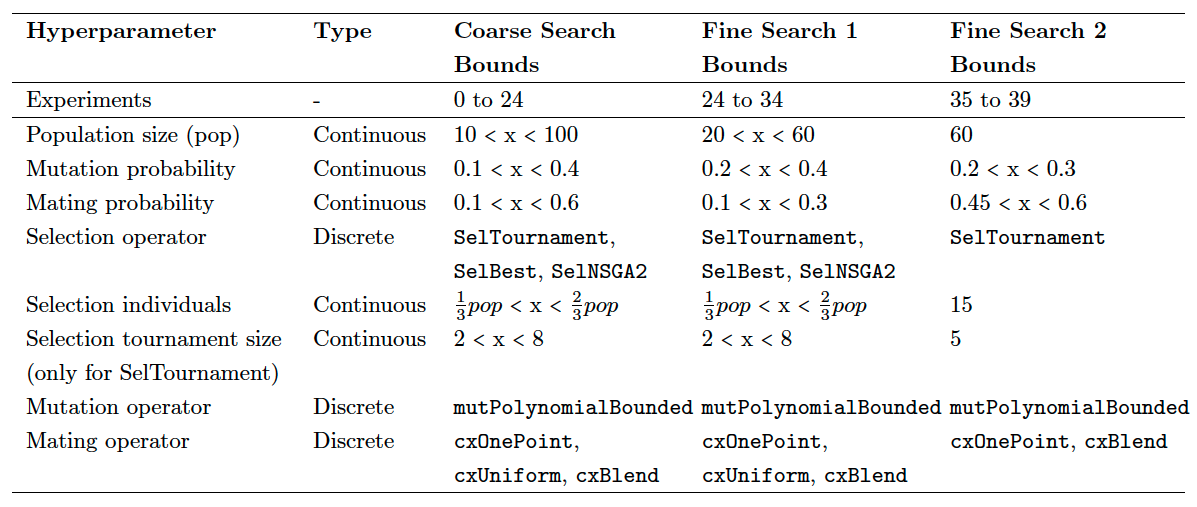
\includegraphics[width=0.8\linewidth]{figures/hyperparameter-search.png} 
    \end{figure}
\end{frame}

\begin{frame}
    \frametitle{Completed Stage II-2: Hyperparameter Search}
    \begin{figure}[]
        \centering
        \makebox[\textwidth][c]{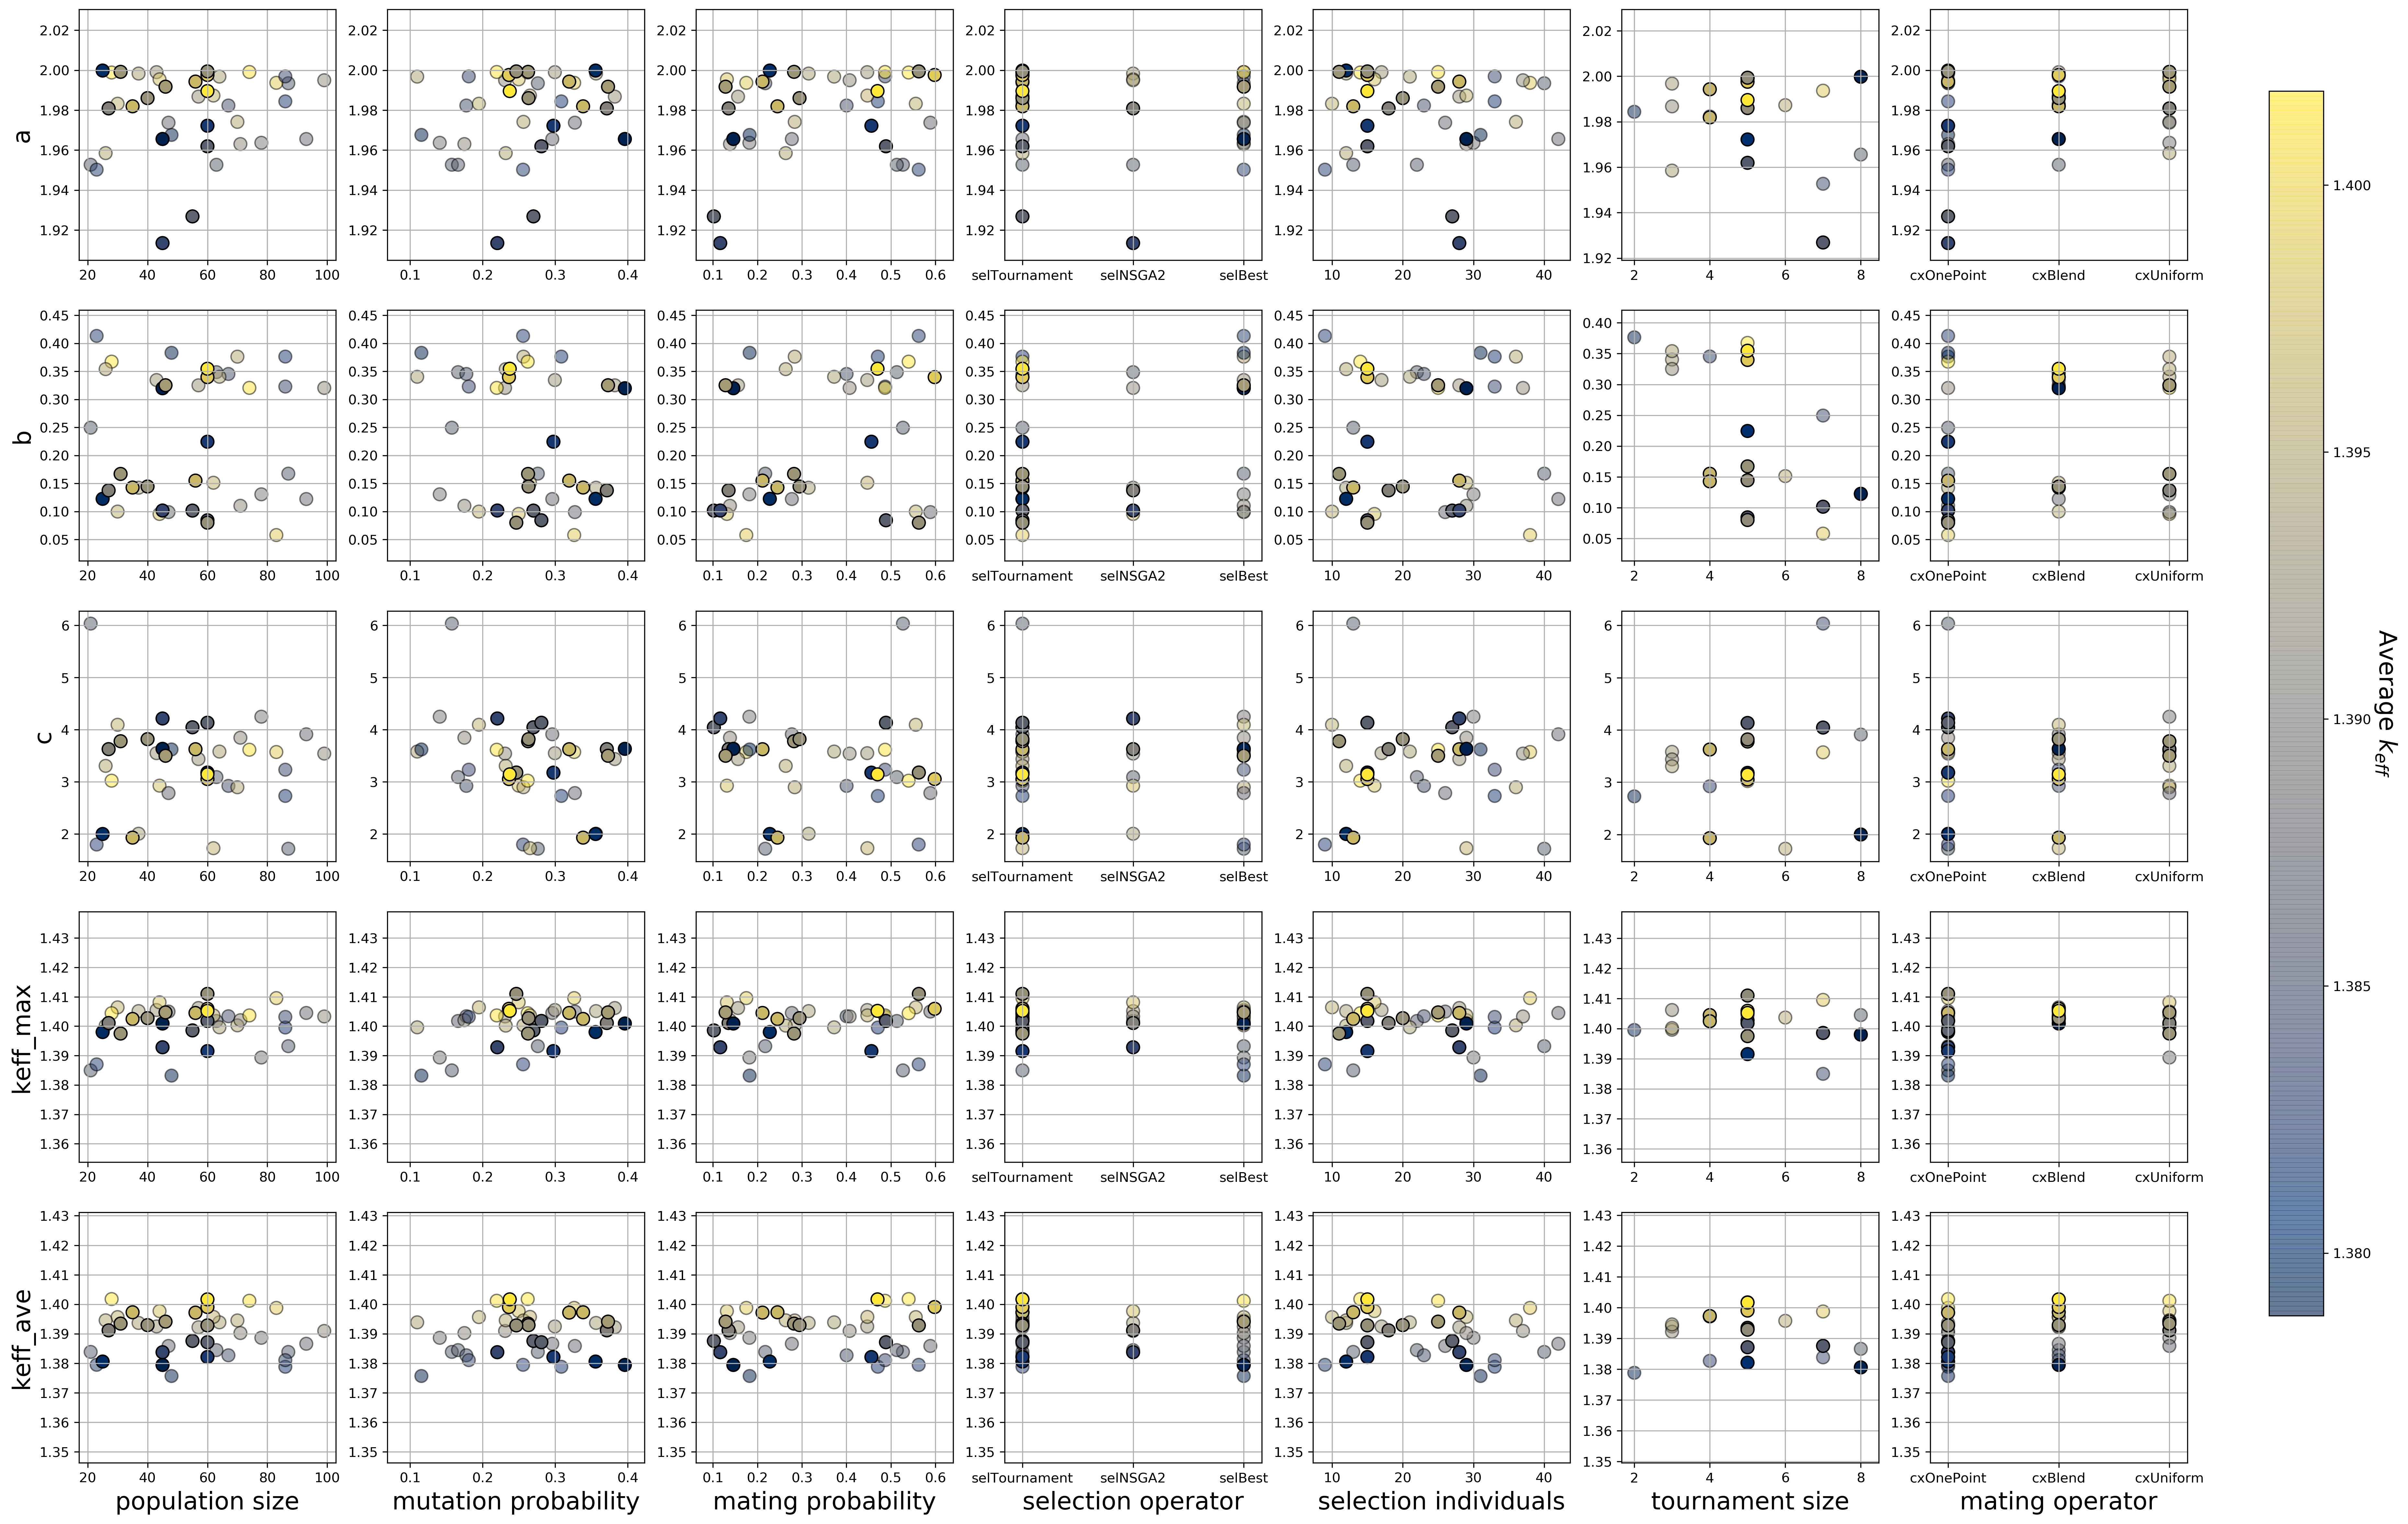
\includegraphics[width=0.65\linewidth]{../docs/figures/input_hyperparameters_sens.png}} 
        \caption{Hyperparameters search's results for all 40 experiments (coarse 
        and fine). I plotted the hyperparameters against: a,b,c control parameters, 
        each experiment's final generation $k_{eff max}$, and final generation 
        $\overline{k_{eff}}$ with a third color dimension representing each experiment's final 
        population's $\overline{k_{eff}}$ (color bar representing the $k_{eff}$ values 
        provided on the right side of the figure). Coarse experiments' (0 to 24) scatter points 
        are $50\%$ transparent, while the fine experiments' (24 to 39) scatter points 
        are opaque.}
    \end{figure}
\end{frame}

\begin{frame}
    \frametitle{Completed Stage II-2: Results from best hyperparameter set}
    \begin{itemize}
        \item I define the best-performing hyperparameter set as the experiment that produces 
        the highest $\overline{k_{eff}}$ in its final generation. 
    \end{itemize}
    \begin{figure}[]
        \centering
        \makebox[\textwidth][c]{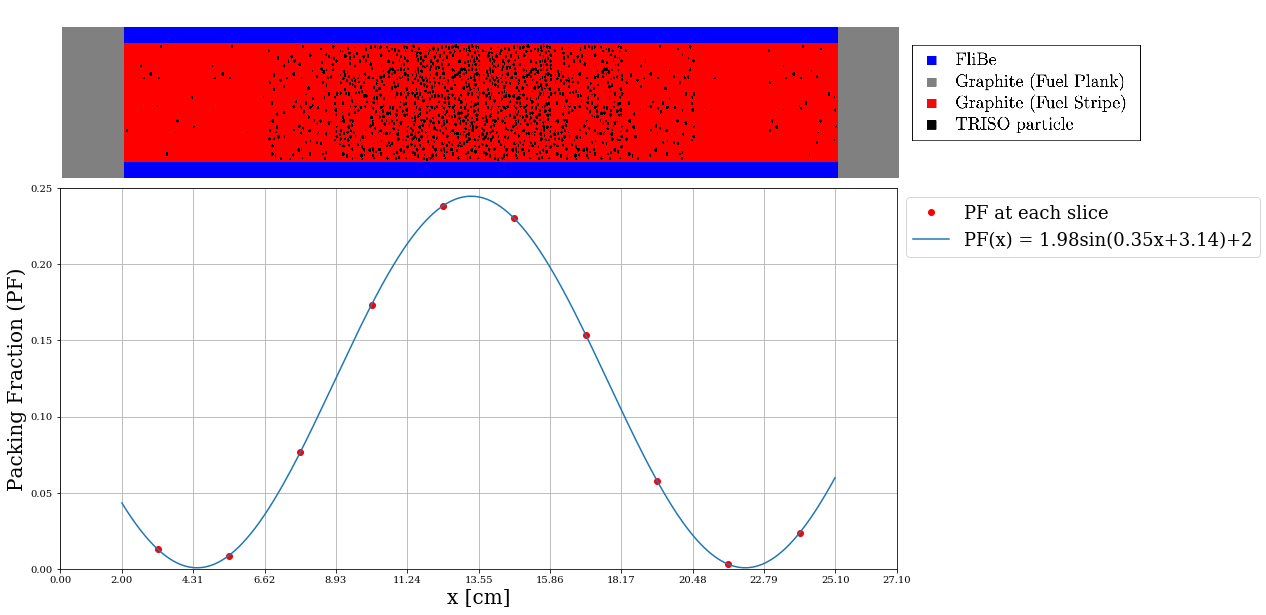
\includegraphics[width=0.75\linewidth]{../docs/figures/triso_distribution_sine_39.png}} 
        \caption{Experiment 39 packing distribution that produced $k_{eff max} = 1.40519 \pm 0.00130$. 
        Below: $PF(x) = (1.98\ sin(0.35x+3.14)+2)  \times NF$ sine distribution with 
        red points indicating the packing fraction at each cell. 
        Above: Straightened AHTR fuel slab with varying TRISO particle 
        distribution across ten cells based on the sine distribution. }
        \label{fig:triso_distribution_sine_39}
    \end{figure}
\end{frame}

\begin{frame}
    \frametitle{Completed Stage II-2: Results from best hyperparameter set}
    \begin{figure}[]
        \centering
        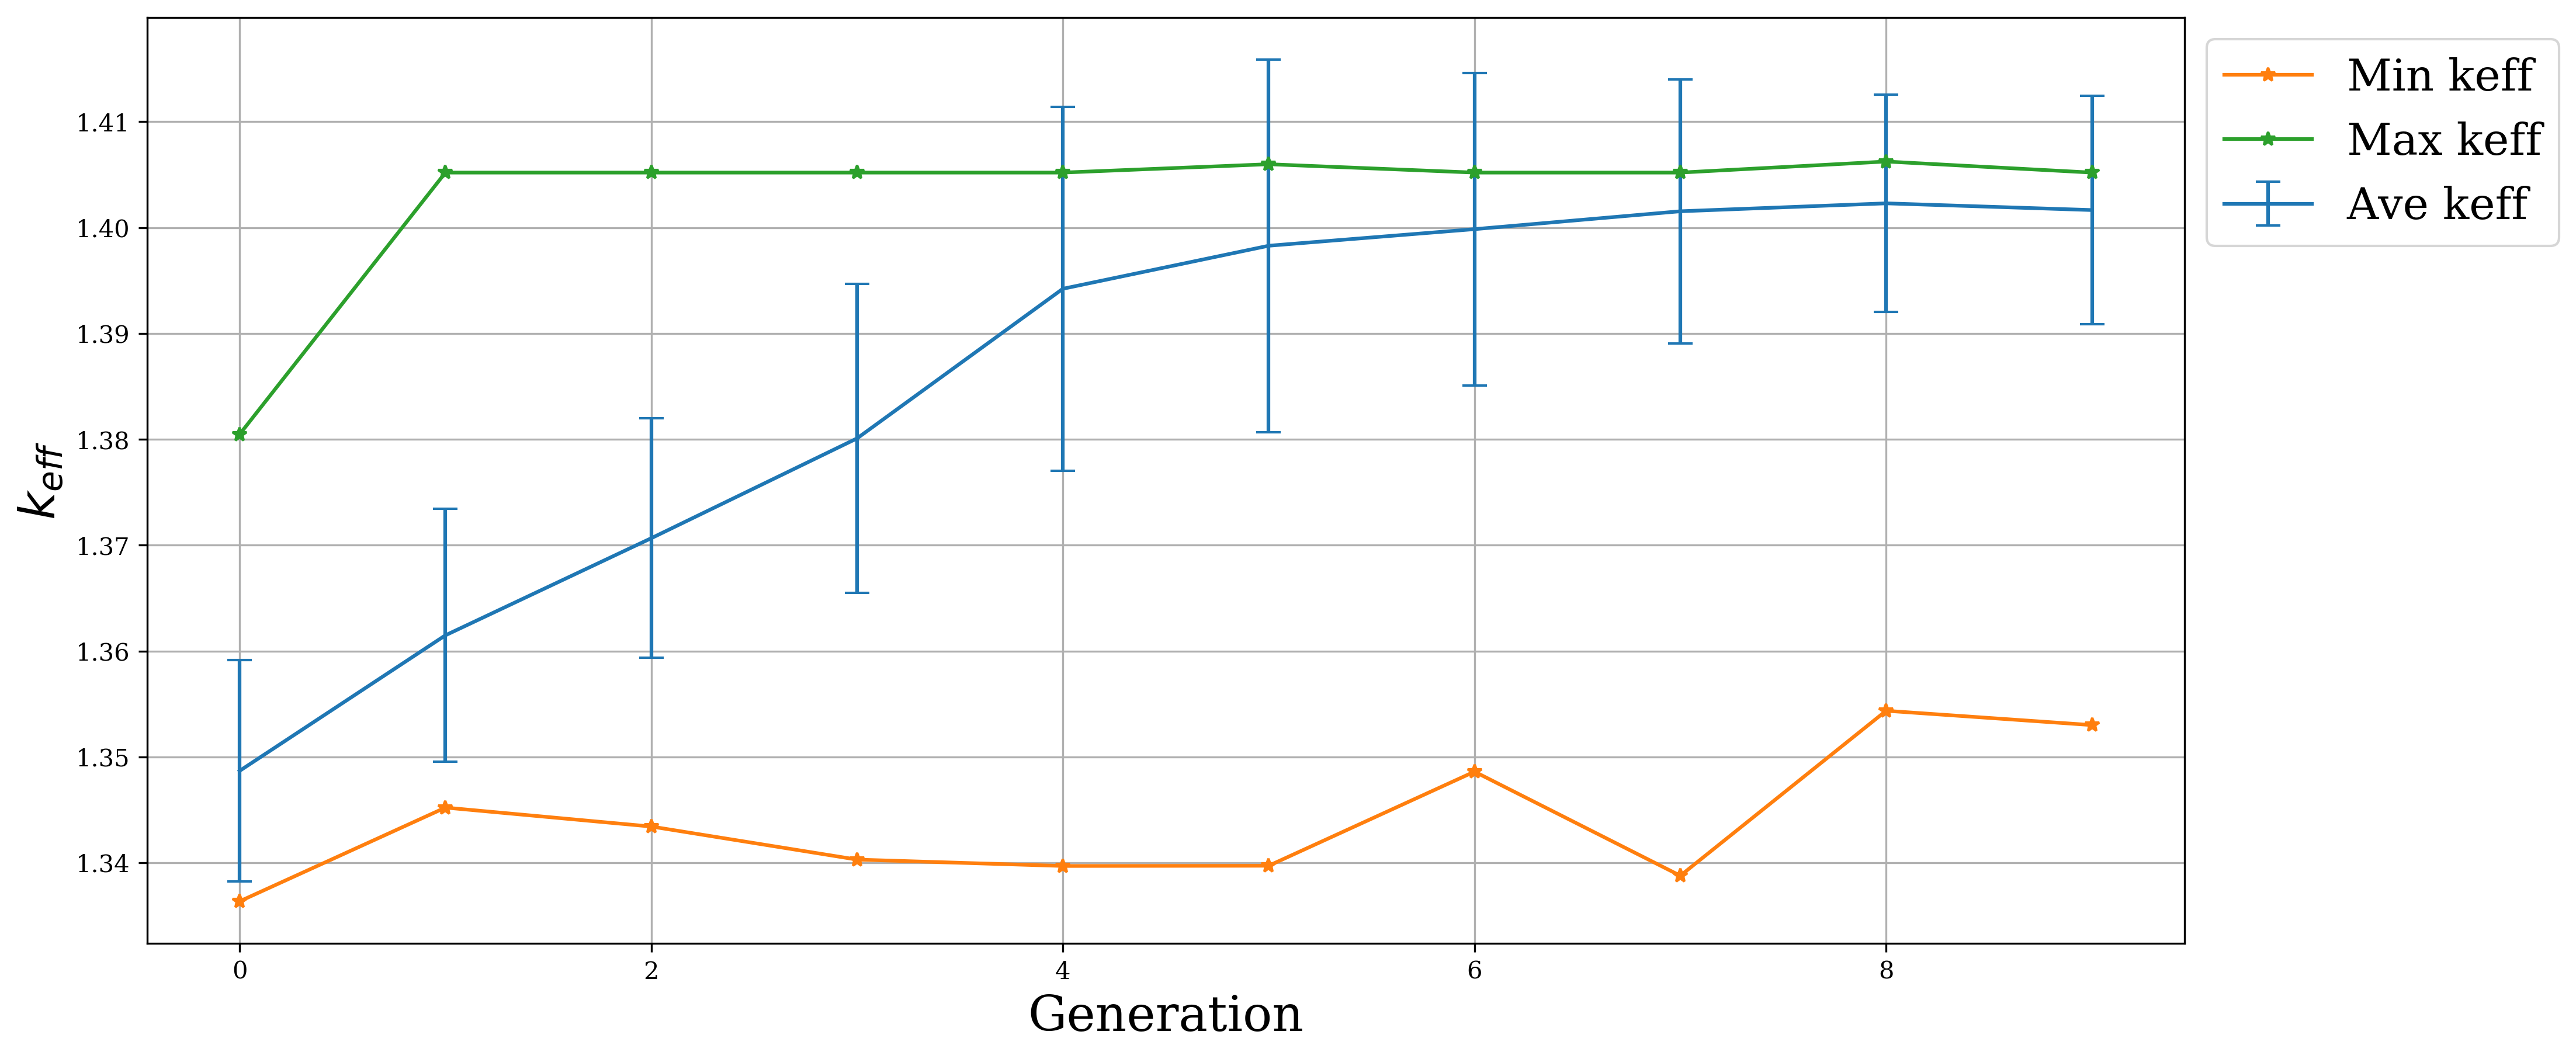
\includegraphics[width=0.55\linewidth]{../docs/figures/keff_conv_39.png}
        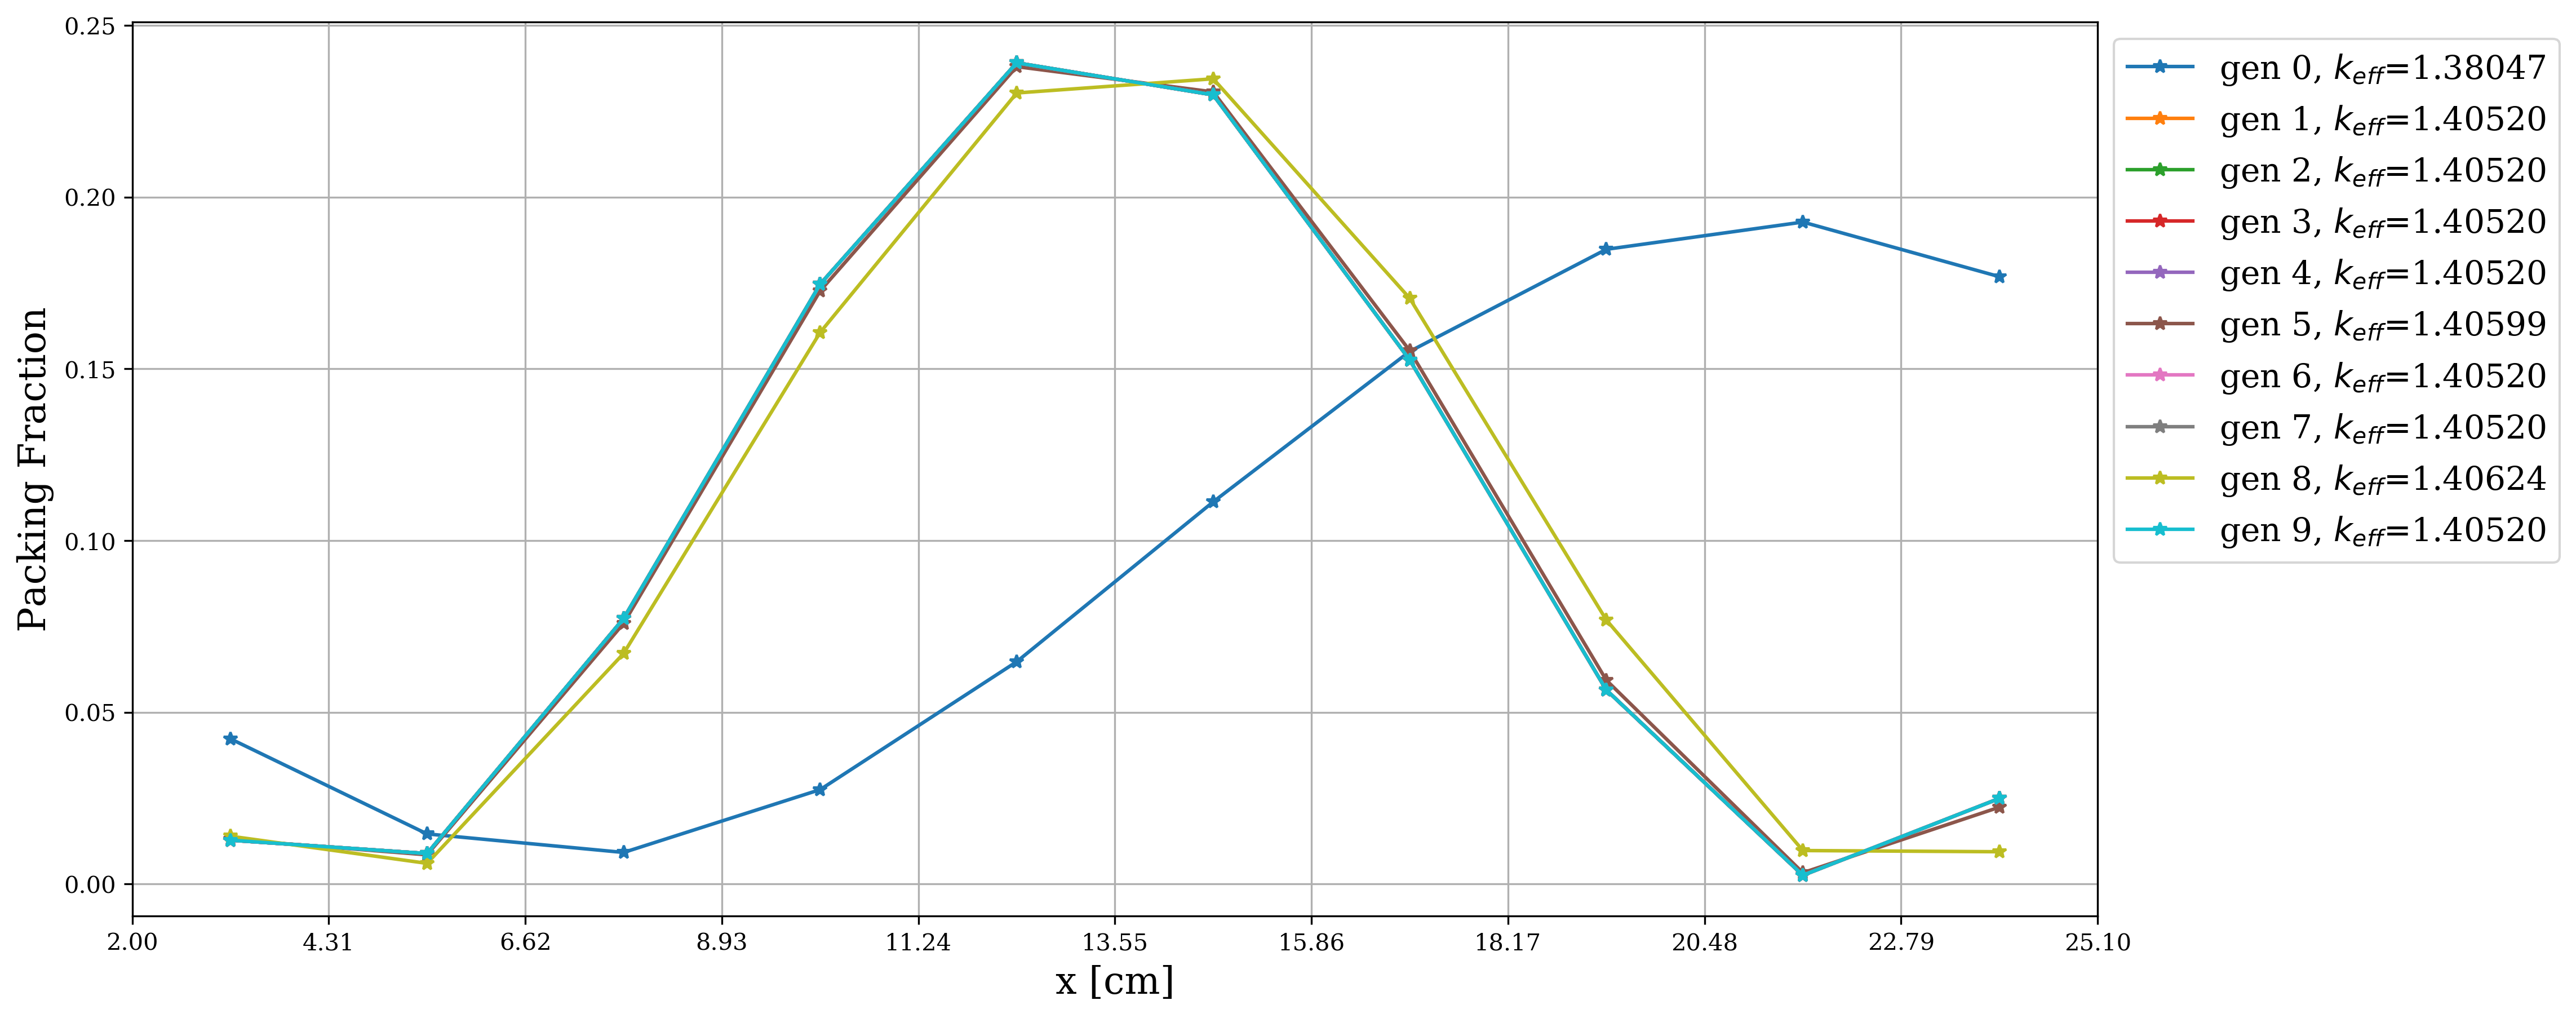
\includegraphics[width=0.55\linewidth]{../docs/figures/pf_39.png}
        \caption{Each generation's results for ROLLO's genetic algorithm 
        optimization of the Straightened \acrfull{AHTR} Fuel Slab. The \gls{ROLLO} 
        simulation used the 39$^{th}$ experiment's hyperparameter set. $k_{eff}$ 
        uncertainty are $\sim$130pcm.}
    \end{figure}
\end{frame}

\subsection{Stage II-3: ROLLO v1.0 Single Objective Problems}
\begin{frame}
    \frametitle{Planned Stage 2-3: ROLLO Single Objective Problems}
    Center-peaking fuel density is nonideal for other key reactor core 
        qualities, such as maximal heat transfer and minimal power peaking factor (PPF).
        Thus, the AHTR slab optimization problem must be extended to include 
        these key reactor core qualities. 
    \begin{block}{Objectives}
        \vspace{-0.2cm}
    \begin{table}
        \caption{ROLLO optimization problem objectives with their quantification 
        descriptions.}
        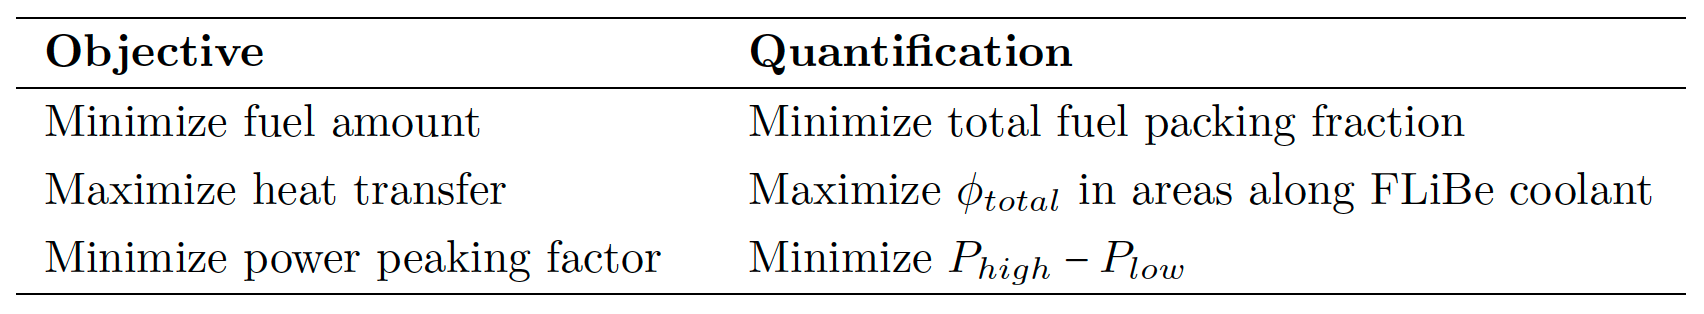
\includegraphics[width=0.7\linewidth]{figures/opt-obj.png}
    \end{table}
\end{block}
\vspace{-0.5cm}
\begin{block}{Control Parameters}
    \begin{itemize}
        \item TRISO particle packing fraction distribution $\rho_{TRISO}(\vec{r})$
        \item Total fuel packing fraction
        \item FLiBe coolant channel shape 
    \end{itemize}
\end{block}
\end{frame}

\begin{frame}
    \frametitle{Planned Stage 2-3: ROLLO Single Objective Problems}
    \begin{table}
        \caption{Proposed ROLLO simulations for AHTR fuel assembly single 
        objective optimization.
        PF: Total Fuel Packing Fraction, $\dot{Q}$: Heat transfer, $PPF$: Power Peaking Factor, 
        $\rho_{TRISO}(\vec{r})$: \gls{TRISO} particle distribution}
        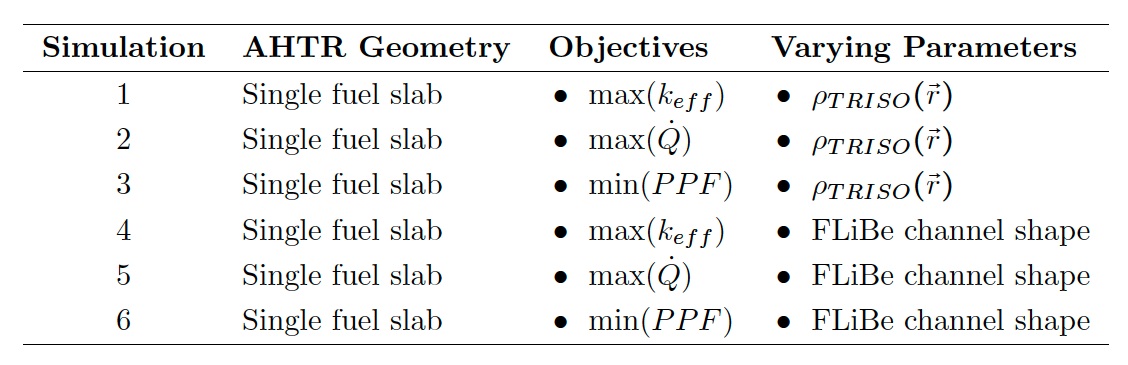
\includegraphics[width=0.8\linewidth]{figures/single-obj.png}
    \end{table}
\end{frame}

\section{Conclusion}

%\input{acks}
%%--------------------------------%%
%%--------------------------------%%
\begin{frame}[allowframebreaks]
  \frametitle{References}
  \bibliographystyle{plain}
  {\footnotesize \bibliography{../docs/2021-chee-prelim.bib} }

\end{frame}

%%--------------------------------%%


\end{document}



